\documentclass{article}

\usepackage[utf8]{inputenc}
\usepackage{amssymb}
\usepackage{amsmath}
\usepackage{amsthm}
\usepackage{amsfonts}
\usepackage{float}
\usepackage{tikz}

\usetikzlibrary{calc}

 \newcommand{\I}{\mathcal{I}}
 \newcommand{\Lmax}{L_{\max}}
 \newcommand{\RR}{\mathcal{R}}
 \newcommand{\DT}{\frac{d}{dt}}

 \newcommand{\DDE}{\frac{D}{d\eta}}

 \newcommand{\DI}{\partial^I}
 \newcommand{\DE}{\partial_{\eta}}
 \newcommand{\NDV}{\frac{\partial_{v}}{R}}
 \newcommand{\NDU}{\frac{\partial_{u}}{R}}
 \newcommand{\DUV}{\partial_{uv}}
 \newcommand{\DUU}{\partial_{uu}}
 \newcommand{\DVV}{\partial_{vv}}

 \newcommand{\Ae}{\text{a.e. }}
 \newcommand{\Csurf}{C_{\text{surf }}}
 \newcommand{\ForAe}{\text{for a.e. }}
 \newcommand{\PLH}{{\mkern-1mu\times\mkern-1mu}}
 \newcommand{\Times}{\PLH}

 \renewcommand{\i}{\mathrm{i}}
\newcommand{\C}{\mathbb{C}}
\newcommand{\R}{\mathbb{R}}
\newcommand{\A}{\mathcal{A}}
\newcommand{\Z}{\mathbb{Z}}
\newcommand{\surf}{M}
\newcommand{\EN}{\mathbb{N}}
\newcommand{\ko}{\kappa}
\newcommand{\kop}{\kappa^{\mathrm{map}}}

\newcommand{\DU}{\partial_{u}}
\newcommand{\DV}{\partial_{v}}
\newcommand{\DerU}{\partial_{u}}
\newcommand{\DerV}{\partial_{v}}
\newcommand{\DerUV}{\partial^2_{uv}}
\newcommand{\DerUU}{\partial^2_{uu}}
\newcommand{\DerVV}{\partial^2_{vv}}

\newcommand{\du}{\mathrm{d}u}
\newcommand{\dx}{\mathrm{d}x}
\newcommand{\dv}{\mathrm{d}v}
\newcommand{\dr}{\mathrm{d}r}
\newcommand{\ds}{\mathrm{d}s}
\newcommand{\dt}{\mathrm{d}t}
\newcommand{\dl}{\mathrm{d}l}
\newcommand{\dz}{\mathrm{d}z}
\newcommand{\modif}[1]{\textcolor{red}{#1}}

\newcommand{\J}{\mathcal{J}}

\newtheorem{theorem}{Theorem}
\newtheorem{lemma}[theorem]{Lemma}
\newtheorem{proposition}[theorem]{Proposition}
\newtheorem{corollaryF}[theorem]{Corollaire}
\newtheorem{definitionF}[theorem]{D�finition}

\newtheoremstyle{prpart}% name of the style to be used
  {\topsep}% measure of space to leave above the theorem. E.g.: 3pt
  {\topsep}% measure of space to leave below the theorem. E.g.: 3pt
  {}% name of font to use in the body of the theorem
  {0pt}% measure of space to indent
  {}% name of head font
  {. }% punctuation between head and body
  { }% space after theorem head; " " = normal interword space
  {\textbf{\thmname{#1} \thmnumber{#2}}\textit{\thmnote{ (#3)}}}
  
\theoremstyle{prpart}
\newtheorem{proofpart}{Step}

\makeatletter
\@addtoreset{proofpart}{theorem}
\makeatother

\newcommand{\CC}{\mathcal{C}}
\renewcommand{\H}{\mathcal{H}}
\newcommand{\B}{\mathcal{B}}
\newcommand*{\Scale}[2][4]{\scalebox{#1}{$#2$}}%

\newcommand{\snum}{\addtocounter{equation}{1}\tag{\theequation}}

 \newcommand{\PU}{\partial_{u}\varphi}
 \newcommand{\PV}{\partial_{v}\varphi}
 \newcommand{\NPU}{{\textstyle\frac{\partial_{u}\varphi}{R}}}

 \newcommand{\Id}{\mathrm{Id}}
\newcommand{\ind}{\mathrm{Ind}}
\newcommand{\hol}{\mathrm{Hol}}
\newcommand{\etaI}{\eta_{\mathrm{set}}}
\newcommand{\gammaI}{\gamma_{\mathrm{set}}}
\newcommand{\st}{g}
\newcommand{\pt}{p}

\begin{document}

\title{Construction of Chebyshev nets with singularities}
\maketitle

\begin{center}{Y.~Masson$^{\textrm{1}}$,
    A.~Ern$^{\textrm{1}}$, L.~Hauswirth$^{\textrm{2}}$,
    L.~Monasse$^{\textrm{1}}$} \end{center}
\begin{center}
  $^{\textrm{1}}$ Universit\'e Paris-Est, CERMICS (ENPC), \\
  6 et 8 avenue Blaise Pascal, Cit\'e Descartes, Champs sur Marne, 77455, Marne la Vall\'ee, Cedex 2, France.
\end{center}
\begin{center}
  $^{\textrm{1}}$ Universit\'e Paris-Est, LAMA, \\
  5 boulevard Descartes, Cit\'e Descartes, Champs sur Marne, 77455, Marne la Vall\'ee, Cedex 2, France.
\end{center}

\bibliographystyle{plain}

\section{Introduction}

\textcolor{red}{A FAIRE !!!}

 
 laurent hauswirth
 
 
 We prove in this chapter the existence and the uniqueness of a Chebyshev net delimited by two smooth curves called boundary conditions. We outline the main ideas of the proof as follows. Following \cite{Ghys09}, we consider the angle distribution defined by the angle between the coordinate curves of the candidate Chebyshev net. We prove that one can construct a unique mapping from this angle distribution such that the $v$-coordinate curves are arc-length parametrized curves with the proper geodesic curvature defined by this angle distribution. Note that the choice of the direction is arbitrary, so that the $u$-coordinate curves could have been chosen. This construction entails a loss of symmetry between these two coordinates which materializes itself by a differentiation between the regularity of the two directions of coordinates curves. The aim is now to view the Hazzidakis formula as a fixed-point equation on the angle distribution, using that the candidate Chebyshev net depends (Lipschitz) continuously on this angle distribution. 

 We then show that, supposing that the Hazzidakis formula is satisfied by the angle distribution, we obtain a regularity pick-up by the use of this identity, and therefore we recover the symmetry between the two directions. Furthermore, we prove that, under suitable regularity conditions, the candidate mapping constructed from the angle distribution is indeed a Chebyshev net, i.e., the $u$-coordinate curves are also arc-length parametrized. The last step of the proof is to show the existence of a unique solution to the equation associated with Hazzidakis formula. This is obtained in the spirit of the Cauchy--Lipschitz theorem: we first prove this existence and uniqueness for a small interval in the $v$-coordinate, and we then extend this result to the whole domain.

\section{Preliminaries}
\subsection{Informal statement of the main result}
Let 
\begin{equation*}
  D=[0,L_u]\Times[0,L_v],\quad\text{with } L_u,L_v\in\R_\ast^+,
\end{equation*}
 and let $\gamma_u:[0,L_u]\to\surf$ and $\gamma_v:[0,L_v]\to\surf$ be two curves such that $\gamma_u(0)=\gamma_v(0)$, and forming an interior angle $\angle(\gamma_u'(0),\gamma_v'(0))\in(0,\pi)$ at their intersection. For clarity of exposition, throughout this chapter, we consider a slightly different notion of Chebyshev net which will refer to mappings (not necessarily homeomorphisms) $\varphi:D\to\surf$ satisfying
\begin{subequations}\label{eq:cheb-def-c3}
\begin{align}\label{eq:cheb-def-c3a}
|\partial_u \varphi|_g(u,v) = 1,\\
|\partial_v \varphi|_g(u,v) = 1,\label{eq:cheb-def-c3b}
\end{align}
\end{subequations}
for all $(u,v)\in D$. Furthermore, note that the orientation of the boundary curve $\gamma_v$ is reversed in this chapter to simplify the exposition. 
We prove in the sequel the existence and the uniqueness of a Chebyshev net $\varphi:D\to\surf$ verifying the primal boundary conditions
\begin{equation}\label{eq:cond-bord-c3}
\begin{split}
  \varphi(u,0)=\gamma_u(u),\quad\forall u\in[0,L_u],\\ 
  \varphi(0,v)=\gamma_v(v),\quad\forall v\in[0,L_v].
\end{split}
\end{equation}
Moreover, we show that the solution depends continuously on these boundary curves, in a sense that will be made precise later on. The considered surface $\surf$ is supposed to be smooth, open, complete, and simply connected and we denote $K$ its Gaussian curvature. %We assume that the total absolute curvature $\int_\surf|K|$ of $\surf$ is finite. 
Due to the above assumptions, the surface $\surf$ is homeomorphic to the plane so that we suppose in what follows that $\surf=(\R^2,g)$. We moreover suppose that the metric $g$ satisfies the following property: for all compact set $W\subset\surf$, there exists $\Csurf>1$ such that 
\begin{equation}\label{eq:equiv}
  |X|_{g(p)} \leq \Csurf|X|,
\end{equation}
for all $p\in W$ and $X\in\R^2$. Unless explicitly mentionned, all the considered curves are assumed to be arc-length parametrized. Then, the geodesic curvature $\ko_{\sigma}:I\subset\R\to\R$ of a curve $\sigma:I\to\surf$ is defined by
\begin{equation}\label{eq:geod-dual1}
   \ko_{\sigma} = \langle\sigma^{\prime\prime},\sigma^{\prime\perp}\rangle_g,
\end{equation}
where $\sigma^{\prime\perp}$ is the direct $\frac{\pi}{2}$-rotation of $\sigma'$. In the sequel, $C$ and $\tilde C$ are two generic constants whose values can change at each occurrence and we will often explicit their dependence.

Following \cite{Ghys09}, we reformulate the problem of finding a Chebyshev net $\varphi:D\to\surf$ as the problem of finding the angle distribution $\omega:D\to\R/2\pi\Z$ between the coordinate curves defined by $\omega(u,v) = \angle(\DU\varphi, \DV\varphi)(u,v)$. With this purpose in mind, we observe that $\omega$ satisfies the following integrability condition (in the form of a modified Sine-Gordon equation) \cite{Ghys09}
\begin{equation}  \label{eq:cond-integr}
  \DUV \omega = -K(\varphi) \sin(\omega).
\end{equation}
Equivalently, $\omega$ satisfies the integrated form of \eqref{eq:cond-integr} called the Hazzidakis formula
\begin{equation}  \label{eq:hazz-form}
\begin{split}
 \omega(u,v) =& ~~\angle\big(\gamma_u'(0),\gamma_v'(0)\big) - \int_0^u \ko_u(s)ds +
  \int_{0}^v\ko_v(s)ds\\
& - \int_0^u\int_0^vK(\varphi(s,t))\sin\big[\omega(s,t)\big]ds~dt,
\end{split}
\end{equation} 
for all $(u,v)\in D$, with $\ko_u:[0,L_u]\to\R$ and $\ko_v:[0,L_v]\to\R$ the geodesic curvatures of $\gamma_u$ and $\gamma_v$ respectively (see Figure \ref{fig:hazz-primal-c4}). 
\begin{figure}[!ht]
  \centering
  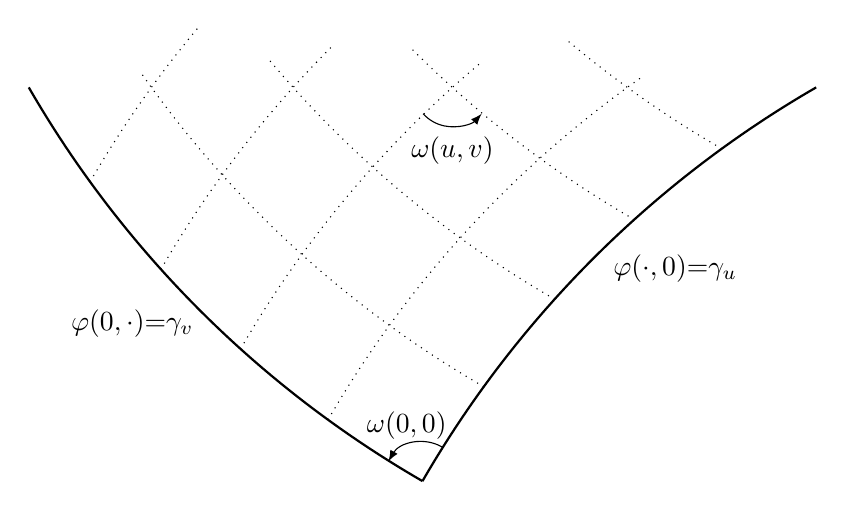
\begin{tikzpicture}[x=1cm,y=1cm]
    \pgfmathsetmacro{\cos}{cos(deg(60))}
    \pgfmathsetmacro{\sin}{sin(deg(60))}
    \draw[thick] (0,0) arc[start angle=150,delta angle=-30,radius=13.66] coordinate[pos=0.2] (u1) coordinate[pos=0.4] (u2) coordinate[pos=0.6] (u3) coordinate[pos=0.8] (u4);
    \coordinate (umid) at (2.3,2.7);
    \draw (umid) node[anchor=west]{$\varphi(\cdot,0){=}\gamma_u$};
    \draw[thick] (0,0) arc[start angle=-120,delta angle=-30,radius=13.66] coordinate[pos=0.2] (v1) coordinate[pos=0.4] (v2) coordinate[pos=0.6] (v3) coordinate[pos=0.8] (v4);
    \coordinate (vmid) at (-2.9,2.);
    \draw (vmid) node[anchor=east,inner sep=0pt]{$\varphi(0,\cdot){=}\gamma_v$};
   \draw[dotted] (u1) arc[start angle=-120,delta angle=-25,radius=13.66];
   \draw[dotted] (u2) arc[start angle=-120,delta angle=-20,radius=13.66];
   \draw[dotted] (u3) arc[start angle=-120,delta angle=-15,radius=13.66] coordinate[pos=0.8] (uv);
   \draw[dotted] (u4) arc[start angle=-120,delta angle=-10,radius=13.66];
   \draw[dotted] (v1) arc[start angle=150,delta angle=-25,radius=13.66];
   \draw[dotted] (v2) arc[start angle=150,delta angle=-20,radius=13.66];
   \draw[dotted] (v3) arc[start angle=150,delta angle=-15,radius=13.66];
   \draw[dotted] (v4) arc[start angle=150,delta angle=-10,radius=13.66];
   \draw[latex-] ($(uv)+(-42:0.5)$) arc[start angle=-42,delta angle=-96,radius=0.5];
   \draw ($(uv)+(-90:0.5)$) node[anchor=north]{$\omega(u,v)$};
 %   \draw[-latex] (0,0) -- (-30:1);
%    \draw ($(0,0)+(-45:0.4)$) node[anchor=north]{$\eta_1'(0)$};
 %   \draw[-latex] (0,0) -- (60:1);
%    \draw ($(0,0)+(130:0.9)$) node[anchor=west, inner sep=1pt]{$\eta_2'(0)$};
%    \draw[-latex] ($(0,0)+(-30:0.5)$) arc[start angle=-30, delta angle=90, radius=0.5];
%    \draw ($(0,0)+(15:0.5)$) node[anchor=west]{$\psi{=}\pi{-}\omega(0,0)$};
    \pgfmathsetmacro{\r}{0.5}
    \draw[-latex] (60:\r) arc[start angle=60, delta angle=90, radius=\r];
    \draw ($(90:.7)+(-.2,0)$) node{$\omega(0,0)$};
  \end{tikzpicture}
  \caption{Illustration of the coordinate curves of a Chebyshev net $\varphi$}\label{fig:hazz-primal-c4}
\end{figure}
We moreover remark that, since $\varphi$ is a Chebyshev net, it satisfies the following property:
\begin{subequations}\label{eq:courb-geod}
\begin{align}\label{eq:courb-geoda}
\kop_u(u,v) &= -\partial_u\omega(u,v), \\\label{eq:courb-geodb}
\kop_v(u,v) &= \partial_v\omega(u,v),
\end{align}
\end{subequations}
for all $(u,v)\in D$, where $\kop_u:D\to\R$ and $\kop_v:D\to\R$ are respectively the geodesic curvatures of the $u$-coordinate curves and of the $v$-coordinate curves of $\varphi$. We obtain by combining \eqref{eq:cond-bord-c3} and \eqref{eq:courb-geod} that the angle distribution $\omega$ satisfies the boundary conditions
\begin{subequations}\label{eq:cond-bord-angle}
\begin{align}
\omega(u, 0) &= \angle(\gamma_u'(0), \gamma_v'(0)) - \int_0^u\ko_u(s)\ds,\quad\forall u\in[0,L_u],\\
\omega(0,v) &= \angle(\gamma_u'(0), \gamma_v'(0)) + \int_0^v\ko_v(s)\ds,\quad\forall v\in[0,L_v].
\end{align}
\end{subequations}
We will first show that we can associate with any angle distribution $\omega:D\to\R/2\pi\Z$ satisfying \eqref{eq:cond-bord-angle} a unique mapping $\varphi:=\I(\gamma,\omega):D\to\surf$ satisfying \eqref{eq:cheb-def-c3b}, \eqref{eq:cond-bord-c3}, and \eqref{eq:courb-geodb}, and then we will show that this mapping also satisfies \eqref{eq:cheb-def-c3a} and \eqref{eq:courb-geoda} whenever $\omega$ satisfies the integrability condition \eqref{eq:cond-integr}. This section aims at proving the following result:
\begin{theorem}[Existence and uniqueness of Chebyshev nets]\label{thm2inexact}
Let $\surf$ be a smooth, open, complete, and simply connected surface. Let $\gamma_u:[0,L_u]\to\surf$, with $L_u\in\R_\ast^+$, and $\gamma_v:[0,L_v]\to\surf$, with $L_v\in\R_\ast^+$, be two curves with respective geodesic curvatures $\ko_u:[0,L_u]\to\R$ and $\ko_v:[0,L_v]\to\R$, and such that $\gamma_u(0) = \gamma_v(0)$. Suppose that $\angle(\gamma_1'(0),\gamma_2'(0))\in(0,\pi)$. Then, there exists a unique angle distribution $\omega:D\to\R/2\pi\Z$, with $D=[0,L_u]\Times[0,L_v]$, verifying the boundary conditions \eqref{eq:cond-bord-angle} and satisfying the Hazzidakis formula \eqref{eq:hazz-form}, with $\varphi:=\I(\gamma,\omega): D\to\surf$ the unique mapping satisfying \eqref{eq:cheb-def-c3b}, \eqref{eq:cond-bord-c3} and \eqref{eq:courb-geodb}.

Suppose moreover that we have $0<\omega(u,v)<\pi$, for all $(u,v)\in D$. Then, $\varphi$ is a Chebyshev net, i.e., it also satisfies \eqref{eq:cheb-def-c3a} and \eqref{eq:courb-geoda}, and the dependency of $\omega$ and $\varphi$ is continuous with respect to the boundary conditions $\gamma_u$ and $\gamma_v$.
\end{theorem}
In the previous statement, we have not defined precisely the regularity of the objects or the norms on the considered vector spaces. These are defined in Section \ref{sec:norms}, and a more accurate statement of Theorem \ref{thm2inexact} is given by Theorem \ref{thm2}. A direct consequence of Theorem \ref{thm2} is the following theorem:
\begin{theorem}[Existence of a unique solution to integrability condition]
  Let $\surf$ be a smooth, open, complete, and simply connected surface. Let $\gamma_u:[0,L_u]\to\surf$, with $L_u\in\R_\ast^+\cup\{\infty\}$, and $\gamma_v:[0,L_v]\to\surf$, with $L_v\in\R_\ast^+\cup\{\infty\}$, be two smooth curves with respective geodesic curvatures $\ko_u:[0,L_u]\to\R$ and $\ko_v:[0,L_v]\to\R$, and such that $\gamma_u(0) = \gamma_v(0)$. Suppose that $\angle(\gamma_u'(0),\gamma_v'(0))\in(0,\pi)$. Then, there exists a unique angle distribution $\omega:D\to\R/2\pi\Z$, with $D=[0,L_u]\Times [0,L_v]$, verifying the boundary conditions \eqref{eq:cond-bord-angle} and satisfying the Hazzidakis formula \eqref{eq:hazz-form}, with $\varphi:=\I(\gamma,\omega): D\to\surf$ the unique mapping satisfying \eqref{eq:cheb-def-c3b}, \eqref{eq:cond-bord-c3} and \eqref{eq:courb-geodb}.

  Suppose moreover that there exists $\tilde D=[0,\tilde L_u]\Times[0,\tilde L_v]$, with $\tilde L_u\in(0,L_u]$ and $\tilde L_v\in(0,L_v]$, such that $0<\omega(u,v)<\pi$, for all $(u,v)\in \tilde D$. Then, the mapping $\varphi\big|_{\tilde D}$ is a Chebyshev nets, that is, it satisfies \eqref{eq:cheb-def-c3} for all $(u,v)\in \tilde D$.
\end{theorem}

In order to prove Theorem \ref{thm2}, we proceed along the following plan. In Section \ref{subsec:constr-param}, given the two curves $\gamma_u$ and $\gamma_v$ on $\surf$ and the angle distribution $\omega:D\to\R/2\pi\Z$ between the coordinate curves, we first construct the candidate Chebyshev net $\varphi=\I(\gamma,\omega):D\to\surf$. We then show that whenever $\varphi$ satisfies the integrability condition \eqref{eq:cond-integr}, this mapping also satisfies \eqref{eq:cheb-def-c3} under suitable regularity conditions.  In Section \ref{subsec:exist-pt-fixe}, we view the Hazzidakis formula \eqref{eq:hazz-form}, with $\varphi:=\I(\gamma,\omega)$, as a fixed-point problem on $\omega$. We show existence and uniqueness of the solution to this fixed-point equation for the curves $\gamma_u$ and $\gamma_v\big|_{[0,L_0]}:[0,L_0]\to\surf$, where $L_0\in(0,L_v]$ is a constant depending on the $C^0$-norm of the geodesic curvatures of $\gamma_u$ and $\gamma_v$. This result is called ``local existence'' in what follows. We finally extend this result to the curves $\gamma_u$ and $\gamma_v$ of arbitrary length, in the spirit of the Cauchy--Lipschitz theorem.

\subsection{Functional spaces and statement of the main result}\label{sec:norms}

We now turn to the regularity required on the curves $\gamma_u$ and $\gamma_v$ and on the angle distribution $\omega$. In what follows, we define the spaces in which the curves, parametrizations and angles are constructed.  %When no confusion is possible, the mention of $L$, $L_u$ and $L_v$ will be dropped in the following notations for the sake of brevity.
Recall that
\begin{equation*}
  D=[0,L_u]\Times[0,L_v],\quad\text{with } L_u,L_v\in\R_\ast^+.
\end{equation*}
Let $k\in\EN$ and $L\in(0,L_v]$. We consider the space $C^{k+2}([0,L],\surf)$ of curves $\gamma$ with general parametrizations on $\surf$ and such that the geodesic curvature of $\gamma$ has $C^{k}$-regularity. % The space $W^{k+2,p}$, endowed with the norm
% \begin{equation}\label{normphi}
%   \|\gamma\|_{W^{k+2,p}} = |\gamma(0)|+|\gamma'(0)| + \|\gamma''\|_{W^{k,p}([0,L])},
% \end{equation}
% is a Banach space.
We define $\Gamma^{k+2}([0,L])$ to be the closed subset of $C^{k+2}([0,L],\surf)$ formed by arc-length parametrized curves:
\begin{equation*}  
  \Gamma^{k+2}([0,L]) = \Big\{\gamma \in C^{k+2}([0,L], \surf) \text{ s.t. } \forall s\in[0,L],~ |\gamma'(s)|_{g(\gamma(s))} = 1\Big\},
\end{equation*}
equipped with the norm $\|\cdot\|_{C^{k+2}([0,L])}$. Note that the norms involved in the Sobolev spaces are the Euclidean norms. Let $r\in\EN$. We define the space $\Theta^{r,k}(D)$ of angle distributions on $D$:
\begin{equation*}
  \Theta^{r,k}(D) = C^r\big([0,L_u],C^k([0,L_v], \R/2\pi\Z)\big),
\end{equation*}
equipped with the norm 
\begin{equation*}
  \|\omega\|_{\Theta^{r,k}(D)} = \|\omega\|_{C^r([0,L_u],C^k([0,L_v]))}.
\end{equation*}
 In the case where $k=r$, the notation of $\Theta^{k,k}(D)$ is simplified to $\Theta^k(D)$. We denote $\Phi^{r,k+2}(D)$ the closed subset of the Banach space $C^r([0,L_u],C^{k+2}([0,L_v],\surf))$ formed by arc-length parametrized curves with $C^{k+2}$-regularity depending on a parameter of regularity $C^r$:
\begin{equation*}  
  \Phi^{r,k+2}(D) := C^r\big([0,L_u], \Gamma^{k+2}([0,L_v])\big)\subset C^r\big([0,L_u],C^{k+2}([0,L_v],\surf)\big).
\end{equation*}
This space is equipped with the norm 
\begin{equation*}
  \|\varphi\|_{\Phi^{r,k+2}(D)} = \|\varphi\|_{C^r([0,L_u],\Gamma^{k+2}([0,L_v]))}.
\end{equation*}
 Note that we do not require the regularity on the first variable to be the same as the regularity on the second variable. This will be made visible in the construction of the candidate Chebyshev net $\varphi$: the first coordinate denotes the initial conditions of an ordinary differential equation in the second coordinate, which does not entail the same regularity.


Let $\gamma=(\gamma_u,\gamma_v)\in\Gamma^{r+2}([0,L_u])\Times \Gamma^{k+2}([0,L_v])$ be two curves with respective geodesic curvatures $\ko_u:[0,L_u]\to\R$ and $\ko_v:[0,L_v]\to\R$, and such that $\gamma_u(0)=\gamma_v(0)$. We define the affine subspace composed of the angle distributions satisfying the boundary conditions \eqref{eq:cond-bord-angle}:
\begin{equation*}  
    \Theta_{\gamma}^{r,k}(D) =
    \left\{ 
      % \begin{array}{c|c} 
      \omega \in \Theta^{r,k}(D),
    % \begin{array}{l}
  %     \displaystyle\omega(u, 0) = \angle(\gamma_u'(0), \gamma_v'(0)) - \int_0^u\ko_u(s)\ds,\\
  %     \displaystyle\omega(0,v) = \angle(\gamma_u'(0), \gamma_v'(0)) + \int_0^v\ko_v(s)\ds
  %   \end{array}\\
  % \end{array}
\text{ s.t. $\omega$ satisfies \eqref{eq:cond-bord-angle}}\right\}.
\end{equation*}
The subspace $\Theta^{r,k}_{\gamma}$ is a closed subset of the Banach space $\Theta^{r,k}$. Again, in the case where $r=k$, we set $\Theta_{\gamma}^k=\Theta_{\gamma}^{k,k}$.

We can now restate Theorem \ref{thm2inexact} with the correct regularity.
\begin{theorem}[Existence and uniqueness of Chebyshev nets]\label{thm2}
Let $\surf$ be a smooth, open, complete, and simply connected surface and let $k\in\EN$. Let $\gamma=(\gamma_u,\gamma_v)\in\Gamma^{k+2}([0,L_u])\Times\Gamma^{k+2}([0,L_v])$, with $L_u,L_v\in\R_\ast^+$, be two curves with respective geodesic curvatures $\ko_u\in C^k([0,L_u])$ and $\ko_v\in C^k([0,L_v])$, and such that $\gamma_u(0) = \gamma_v(0)$. Suppose that $\angle(\gamma_1'(0),\gamma_2'(0))\in(0,\pi)$. Then, there exists a unique angle distribution $\omega:=\J(\gamma) \in \Theta^{k+1}_{\gamma}(D)$, with $D=[0,L_u]\Times[0,L_v]$, verifying the boundary conditions \eqref{eq:cond-bord-angle} and satisfying the Hazzidakis formula \eqref{eq:hazz-form}, with $\varphi:=\I(\gamma,\omega)\in\Phi^{k+2}(D)$ the unique mapping satisfying \eqref{eq:cheb-def-c3b}, \eqref{eq:cond-bord-c3} and \eqref{eq:courb-geodb}. 

Suppose moreover that we have $0<\omega(u,v)<\pi$, for all $(u,v)\in D$. Then, $\varphi$ is a Chebyshev net, i.e., it also satisfies \eqref{eq:cheb-def-c3a} and \eqref{eq:courb-geoda}, and the mappings
\begin{equation*}
\begin{array}{cccc}
\J:&\Gamma^{k+2}([0,L_u])\Times\Gamma^{k+2}([0,L_v])&\to&\Theta^{k+1}(D),\\
  \I:&\Gamma^{k+2}([0,L_u])\Times\Gamma^{k+2}([0,L_v])\Times\Theta^{k+1}(D)&\to&\Phi^{k+2}(D)
\end{array}
\end{equation*}
are continuous.
\end{theorem}

\section{Construction of a Chebyshev net from its angle distribution}\label{subsec:constr-param}
We now prove that a Chebyshev net can be constructed uniquely from its angle distribution. We start by showing in Subsection \ref{subsec:construction} that the construction of curves from their geodesic curvature, initial point and initial tangent vector is a well-posed problem. We then define, following \cite{Ghys09}, the mapping $\I(\gamma,\omega)$ which, for given boundary curves $\gamma_u$ and $\gamma_v$, associates with any angle distribution $\omega$ satisfying the boundary conditions \eqref{eq:cond-bord-angle} the candidate Chebyshev net $\varphi$, with angle distribution $\omega$, satisfying the boundary conditions \eqref{eq:cond-bord-c3} (Subsection \ref{subsubsec:constr-param}). The parametrization $\varphi$ is constructed in such a way that the $v$-coordinate curves are arc-length parametrized curves with geodesic curvatures satisfying \eqref{eq:courb-geodb}. We moreover show the continuity of the mapping $\I$ with respect to the angle distribution and to the delimiting curves $\gamma_u$ and $\gamma_v$. In Subsection \ref{sec:reg-candidate}, we show that the candidate Chebyshev net $\varphi$ has improved regularity in the $u$-coordinate whenever $\omega$ satisfies the integrability condition \eqref{eq:cond-integr}. Finally, in Subsection \ref{sec:reg-cheb}, we prove that $\varphi$ is indeed a Chebyshev net if $\omega$ satisfies the integrability condition and has a sufficient regularity.

\subsection{Construction of curves from their geodesic curvature}\label{subsec:construction}
\begin{proposition}[Construction of curves from their geodesic curvature]\label{prop:constr-courbe}
 Let $\surf$ be a smooth, open, complete, and simply connected surface. Let $\Lmax\in\R^+_\ast$, $L\in(0,\Lmax)$ and $k,r\in\EN$. Let $x\in \surf$, let $V\in T_x\surf$ be a unit vector, i.e., a vector such that $|V|_g=1$, and let $\ko\in C^k([0,L],\R)$. Then, there exists a unique (arc-length parametrized) curve $\sigma(x,V,\ko):=\sigma\in \Gamma^{k+2}([0,L])$ such that $\sigma(0) = x$, $\sigma'(0) = V$, and with geodesic curvature $\ko$.

  Moreover, let $L_1,L_2\in(0,\Lmax)$, let $x_1,x_2\in C^r([0,L_1],\surf)$ be initial position distributions and let $V_1,V_2\in C^r([0,L_1],T\surf)$, with $|V_1|_g=|V_2|_g=1$, be initial derivatives distribution. Let $D_{1,2}=[0,L_1]\Times[0,L_2]$ and let $\ko_1, \ko_2 \in C^r([0,L_1],C^k([0,L_2],\R))$ be geodesic curvatures. We denote $\sigma_1,\sigma_2:[0,L_1]\to \Gamma^{k+2}([0,L_2])$ the two families of curves defined by $\sigma_m(\eta,\cdot):=\sigma(x_m(\eta),V_m(\eta),\ko_m(\eta,\cdot))$, for all $\eta\in[0,L_1]$ and $m\in\{1,2\}$. Then, we have
\begin{equation*}
\sigma_1,\sigma_2\in \Phi^{r,k+2}(D_{1,2})=C^r([0,L_1],\Gamma^{k+2}([0,L_2])),
\end{equation*}
and, for all $m\in\{1,2\}$, 
\begin{equation}\label{eq:borne-courbe}
\begin{split}
\|\sigma_m\|_{\Phi^{r,k+2}(D_{1,2})} \leq C,
\end{split}
\end{equation}
where the constant $C$ depends on $\Lmax$, $\|x_m\|_{C^r([0,L_1])}$, $\|V_m\|_{C^r([0,L_1])}$, and $\|\ko_m\|_{C^r([0,L_1],C^k([0,L_2]))}$.
Finally, we have%, for all $1\leq p\leq\infty$,
\begin{subequations}  \label{eq:estim-courbe}
\begin{align}\label{eq:estim-courbe1}
\begin{split}
  \|\sigma_1-\sigma_2\|_{\Phi^{0}(D_{1,2})} &\leq C\Big(L_2\|\ko_1-\ko_2\|_{C^0(D_{1,2})} \\
&  \quad+ \|x_1-x_2\|_{C^0([0,L_1])}+\|V_1-V_2\|_{C^0([0,L_1])}\Big),
\end{split}\text{ if $k=0$ and $r=0$,}\\\label{eq:estim-courbe2}
\begin{split}
  \|\sigma_1-\sigma_2\| _{\Phi^{r,k+2}(D_{1,2})}& \leq \tilde C\Big(\|\ko_1-\ko_2\|_{C^r([0,L_1],C^k([0,L_2]))} \\
  &\qquad+ \|x_1-x_2\|_{C^r([0,L_1])}+\|V_1-V_2\|_{C^r([0,L_1])}\Big),
\end{split}
\end{align}
\end{subequations}
where the constants $C$ and $\tilde C$ depend on $\Lmax$, $\|x_m\|_{C^r([0,L_1])}$, $\|V_m\|_{C^r([0,L_1])}$, and $\|\ko_m\|_{C^r([0,L_1],C^k([0,L_2]))}$, with $m\in\{1,2\}$.
\end{proposition}
We illustrate the family of curves $\sigma_1$ introduced in Proposition \ref{prop:constr-courbe} in Figure \ref{fig:construction}.
\begin{figure}[!ht]
  \centering
  \begin{tikzpicture}[x=1.8cm,y=1.8cm]
    \draw[red] (0,0) node[anchor=north east,inner sep=1pt]{$x_1(0)$};
    \draw[red] (0,0) node{$\times$};
    \draw[thick,red] (0,0) arc[start angle=110,delta angle=-40,radius=5] coordinate[pos=0.5] (v1) coordinate[pos=0.3] (v2);
    \draw[thick] (0,0) arc[start angle=200,delta angle=-40,radius=5] coordinate[pos=0.5] (v3);
    \draw (v3) node[anchor=east]{$\sigma_1(0,\cdot)$};
    \draw (v2) arc[start angle=180,delta angle=-40,radius=5] coordinate[pos=0.5] (v4)  coordinate[pos=0.7] (v5);
    \draw (v4) node[anchor=east]{$\sigma_1(\eta,\cdot)$};
    \draw[red] (v2) node[anchor=north]{$x_1(\eta)$};
    \draw[red] (v2) node{$\times$};
    \draw[-latex,red] (v2) -- ($(v2)+(90:.6)$) node[pos=0.4,anchor=south east]{$V_1(\eta)$};
    \draw[-latex,red] (0,0) -- ($(110:.6)$) node[pos=0.4,anchor= east]{$V_1(0)$};
    \draw (v5) node[anchor=east]{$\sigma_1(\eta,s)$};
    \draw (v5) node{$\times$};
   \end{tikzpicture}
  \caption{Illustration of the construction of the family of curves $\sigma_1$}\label{fig:construction}
\end{figure}
\begin{proof}
  To prove the claim, we proceed as follows. We first introduce in Step \ref{step:geod-eq} the geodesic curvature equation that permits to define uniquely a curve from its geodesic curvature. The existence and the uniqueness of the curve is proved in Step \ref{step:init-induc} using Cauchy--Lipschitz theorem. Then, in order to apply an induction argument, we prove \eqref{eq:borne-courbe} and \eqref{eq:estim-courbe} in the case $k=0$ and $r=0$ using Grönwall's inequality. The equation satisfied by the derivatives of the solution is presented in a generic form to facilitate the end of the proof in Step \ref{step:diff-eq}. Finally, we prove \eqref{eq:borne-courbe} and \eqref{eq:estim-courbe2} in Steps \ref{step:borne} and \ref{step:control} using induction arguments. Whenever there is no ambiguity, the domain of the variables will be omitted.
  \begin{proofpart}[Formulation of the geodesic curvature equation]\label{step:geod-eq}
  Let $(\sigma^1,\sigma^2)$, with $\sigma^1,\sigma^2:[0,L]\to\R$, be the coordinates of the candidate curve $\sigma:[0,L]\to\surf$ with geodesic curvature $\ko$. %The proof follows directly by application of Carathéodory's existence theorem \cite{Har64}, Grönwall's and Jensen's inequalities on
 We denote $\frac{D}{dt}$ the covariant derivative along the curve $\sigma$. The geodesic curvature equation for arc-length parametrized curves gives
\begin{equation}
\label{eq:geod-curv}
  \frac{D}{dt}\sigma' = \ko\sigma^{\prime\perp},
\end{equation}
which can be written, in coordinates,
\begin{equation}
\label{eq:pr-edo}
  \dot X = G(X) + \ko f(X),
\end{equation}
with $X(0)=(x^1,x^2,V^1,V^2)$. Here, we have denoted
\small
\begin{equation*}
  X = 
\left(
\begin{array}{c}
\sigma^1\\\sigma^2\\\sigma^{\prime 1}\\\sigma^{\prime 2} 
\end{array}\right), \quad
f(X) = \left( 
  \begin{array}{c}
    0\\0\\N^1\\N^2
    \end{array} \right), \quad
G(X) = \left(
  \begin{array}{c}
    X^3\\ X^4\\\displaystyle -\sum_{1\leq i,j\leq 2}\Gamma_{i,j}^1(X^1,X^2)X^{2+i}X^{2+j}\\ 
\displaystyle-\sum_{1\leq i,j\leq 2}\Gamma_{i,j}^2(X^1,X^2)X^{2+i}X^{2+j}
  \end{array}\right),
\end{equation*}
\normalsize
$\Gamma_{ij}^{k}$ being the smooth Christoffel symbols, $G$ the smooth geodesic function and $N$ the normal vector defined by
\begin{equation*}
N = \left(\begin{array}{c}
N^1\\N^2
\end{array}\right)
= \sqrt{\det g(X^1,X^2)}g^{-1}(X^1,X^2)
  \left(\begin{array}{c}
      -X^4\\X^3
      \end{array}\right).
\end{equation*}
%We prove the assertions of the proposition by induction on $k\geq0$ and $r\geq0$.
\end{proofpart}

\begin{proofpart}[Proof for $k=0$ and $r=0$]\label{step:init-induc}
%\paragraph*{Proof for $k=0$ and $r=0$.}
  As $G+\ko f$ is continuous and locally Lipschitz continuous with respect to $X$, owing to Cauchy--Lipschitz theorem, there exists a local solution to \eqref{eq:pr-edo}. Moreover, since $\sigma$ is by construction arc-length parametrized, we have $|\sigma'|_g=1$ and we infer from \eqref{eq:equiv} that $|\sigma'|\leq\Csurf$. Hence, the image of $X$ is included in a ball $\B$ whose radius depends only on $\Lmax$ and $\Csurf$. We deduce that the solution is defined on $[0,L]$. Moreover, $G$ and $f$ are Lipschitz continuous with respect to $X$ on $\B$. Hence, $G+\ko f$ is Lipschitz continuous with respect to $X$ on $\B$, so that the uniqueness of the solution follows. Moreover, we infer from \eqref{eq:pr-edo} that $\sigma\in\Gamma^{2}([0,L])$.

  Let $m\in\{1,2\}$ and let $X_m = (\sigma_m^1, \sigma_m^2, \sigma_m^{\prime 1}, \sigma_m^{\prime 2})^t:D_{1,2}\to\R^4$ be such that $X_m(\eta,\cdot)$ is the unique solution to \eqref{eq:pr-edo} with $\ko=\ko_m(\eta,\cdot)$, for all $\eta\in[0,L_1]$. First, owing to \cite[Chap. V, Th. 2.1]{Har64}, we have $X_m\in C^0([0,L_1], C^1([0,L_2]))$, so that $\sigma_m\in \Phi^{0,2}(D_{1,2})$. Then, since $|\sigma'|\leq\Csurf$, we infer that $\|\sigma_m\|_{\Phi^{0,2}(D_{1,2})}\leq C$, where the constant $C$ depends on $\|\sigma_m(\cdot,0)\|_{C^0([0,L_1])}$ and $\|X_m'\|_{C^0(D_{1,2})}$. Moreover, due to $|f(X_m)|_g = |\sigma_m'|_g=1$, we have
  \begin{equation}\label{eq:pr-bound-f}
    |f(X_m)|\leq \Csurf.
  \end{equation}
Furthermore, since $X_m(\{\eta\}\times[0,L_2])\subset \B$, we infer that $G(X_m)$ is bounded and that this bound only depends on $\B$, so that it only depends on $X_m(\eta,0)$, $\Lmax$ and $\Csurf$, for all $\eta\in[0,L_1]$. We conclude that
\begin{equation*}
  \|\sigma_m\|_{\Phi^{0,2}(D_{1,2})}\leq C,
\end{equation*}
where the constant $C$ depends on $\|x_m\|_{C^0([0,L_1])}$ and $\|\ko_m\|_{C^0(D_{1,2})}$, and \eqref{eq:borne-courbe} holds with $k=r=0$.
Then, since the restrition of $G$ and $f$ to $\B$ are Lipschitz continuous in the variable $X$ with coefficients denoted respectively $C_G$ and $C_f$, we have  
\begin{equation*}
  |\dot X_1 - \dot X_2| \leq (C_G+|\ko_1| C_f)|X_2-X_1|+|\ko_2-\ko_1| \ \|f(X_2)\|_{C^0(D_{1,2}))}.
\end{equation*} 
Therefore, using Grönwall's inequality and \eqref{eq:pr-bound-f}, we infer that
\small
\begin{equation}
 \label{eq:reg-equ-geod}
 |X_1(t)-X_2(t)| \leq
  \exp\Big[t\big(C_G+C_f \|\ko_1\|_{C^0(D_{1,2})}\big)\Big]\left(|X_2(0) - X_1(0)| + \Csurf\int_0^t \left|\ko_2 - \ko_1\right| \right),
\end{equation}
\normalsize
for all $t\in[0,L]$. We deduce that \eqref{eq:estim-courbe1} and \eqref{eq:estim-courbe2} are satisfied for $k=r=0$. % and $p=\infty$. 
% Now, suppose that $1\leq p<\infty$. By Jensen's inequality and \eqref{eq:reg-equ-geod}, we have 
% \begin{align*}
%   |X_1(t)-X_2(t)|^p &\lesssim |X_2(0) - X_1(0)|^p + \Big(\int_0^t \left|\ko_2 - \ko_1\right|\Big)^p \\
%   &\lesssim |X_2(0) - X_1(0)|^p + t^{p-1}\int_0^t \left|\ko_2 - \ko_1\right|^p.
% \end{align*}
% We easily conclude that \eqref{eq:estim-courbe1} and \eqref{eq:estim-courbe2} are satisfied with $k=0$, $r=0$ and $p<\infty$.
\end{proofpart}

\begin{proofpart}[Differential equation on the derivatives of $X$]\label{step:diff-eq}
%\paragraph*{Differential equation on the derivatives of $X$.}
Let $m\in\{1,2\}$. Owing to \cite[Chap. V, Th. 4.1]{Har64}, we have that $\sigma\in \Gamma^{k+2}([0,L])$ and $\sigma_m\in \Phi^{r,k+2}(D_{1,2})$.
We use the following notation: for $I=(i_1,i_2)\in \EN^2$, we set $\DI f(\eta,t) = \partial_\eta^{i_1}\partial^{i_2}_t f(\eta,t)$. 
We denote $(\H_{r,k})$, with $r,k\in\EN^\ast$, the following induction hypothesis:

\textit{for all $I=(i_1,i_2)\in\{0,...,r\}\Times\{0,...,k\}$ such that $I\neq (0,0)$, we have
\begin{equation}\label{eq:eq-der-courbe}
\begin{split}
\partial_t \DI X_m = &~~(\nabla G(X_m)+\ko_m\nabla f(X_m))\DI X_m \\
&+ \sum_{0\leq\alpha\leq i_1}\sum_{0\leq\beta\leq i_2}F^I_{\alpha,\beta}\left[(\partial^{(p,q)}X_m)_{0\leq p+\alpha \leq i_1,~0\leq q+\beta\leq i_2,~p+q<i_1+i_2}\right] \partial^{(\alpha,\beta)}\ko_m,
\end{split}
\end{equation}
where $F^I_{\alpha,\beta}:\R^{4n_0}\to \R^4$, with
\begin{equation*}
 n_0=\left\{\begin{split}
 &(i_1-\alpha+1)(i_2-\beta+1), &\quad\text{if } \alpha+\beta\neq0,\\
  &(i_1+1)(i_2+1)-1, &\quad\text{otherwise},
\end{split}\right.
\end{equation*}
are $C^\infty$ functions, for all $(\alpha,\beta)\in\{0,...,i_1\}\Times\{0,...,i_2\}$. %Moreover, $F^I_{\alpha,\beta}$ is polynomial in $\partial^{(p,q)}X_m$, with $(p,q)\in\{0,...,i_1-\alpha\}\Times\{0,...,i_2-\beta\}$ such that $(p,q)\neq(0,0)$, for all $(\alpha,\beta)\in\{0,...,i_1\}\Times\{0,...,i_2\}$.
}

We denote $\partial_1$ and $\partial_2$ the derivatives with respect to $\eta$ and $t$ respectively. We first obtain from \eqref{eq:pr-edo} that,
 for all $m\in\{1,2\}$ and $i\in\{1,2\}$, 
\begin{equation*}
 \partial_t \partial_i X_m = \nabla G(X_m)\partial_i X_m 
 + \partial_i \ko_m f(X_m) + \ko_m\nabla f(X_m) \partial_i X_m.
\end{equation*}
Hence, \eqref{eq:eq-der-courbe} is satisfied for $I=(0,1)$ and $I=(1,0)$, so that $(\H_{1,1})$ holds. We now suppose that $(\H_{r,k})$ holds for $r,k\in\EN^\ast$. Then, for $I=(i_1,i_2)$ with $i_1=r$ and $i_2=k$, we have 
\begin{align*}
\partial_t\partial_i\DI X_m &= (\nabla G(X_m)+\ko_m\nabla f(X_m))\partial_i\DI X_m + \partial_i\big[\nabla G(X_m)+\ko_m\nabla f(X_m)\big]\DI X_m \\
&\quad+ \sum_{0\leq\alpha\leq i_1}\sum_{0\leq\beta\leq i_2}\bigg[\partial_i \left(F^I_{\alpha,\beta}\left[(\partial^{(p,q)}X_m)_{0\leq p+\alpha \leq i_1,~0\leq q+\beta\leq i_2, ~p+q<i_1+i_2}\right]\right) \partial^{(\alpha,\beta)}\ko_m \\
  &\qquad\qquad\qquad\qquad\quad+ F^I_{\alpha,\beta} \partial_i\partial^{(\alpha,\beta)}\ko_m\bigg].
\end{align*}
The first term is in the form of the first term on the right-hand side of \eqref{eq:eq-der-courbe} and the last two terms can be put in the form of the second term on the right-hand side of \eqref{eq:eq-der-courbe}. Equation \eqref{eq:eq-der-courbe} is then satisfied for $I=(r+1,k)$ and $I=(r,k+1)$, so that $(\H_{r+1,k})$ and $(\H_{r,k+1})$ hold. The claim follows.
\end{proofpart}

\begin{proofpart}[Proof of \eqref{eq:borne-courbe}]\label{step:borne}
%\paragraph*{Proof of \eqref{eq:borne-courbe}.}
Let $m\in\{1,2\}$. First note that we have by definition
\begin{align*}
\|\sigma_m\|_{\Phi^{r,k+2}(D_{1,2})} &\leq  \sum_{i_1=0}^{r}\sum_{i_2=0}^{k+1}\|\partial_{\eta}^{i_1}\partial_{t}^{i_2}X_m\|_{C^0(D_{1,2})}.
\end{align*}
Then, to obtain \eqref{eq:borne-courbe}, we only need to prove that
\begin{equation}\label{eq:pr-borne-courbe}
  \|\DI X_m\|_{C^0(D_{1,2})} \leq C,
\end{equation}
where the constant $C$ depends on $\Lmax$, $\|x_m\|_{C^{i_1}([0,L_1])}$, $\|V_m\|_{C^{i_1}([0,L_1])}$, and $\|\ko_m\|_{C^{i_1}([0,L_1],C^{i_2}([0,L_2]))}$,
for all $I=(i_1,i_2)\in\{0,...,r\}\Times\{0,...,k{+}1\}$. We prove \eqref{eq:pr-borne-courbe} by induction on $I\in\{0,...,r\}\Times\{0,...,k+1\}$. Hence, we first consider the case $i_2=0$, in which case we have, using \eqref{eq:eq-der-courbe} and Grönwall's inequality,
\begin{equation*}
\begin{split}
|\partial_\eta^{i_1}X_m(t)|\leq&\exp\big[\|\nabla G(X_m) +\ko_{\sigma_m}\nabla f(X_m)\|_{C^0(D_{1,2})}t\big]\\
&\Times\Big(|\partial_\eta^{i_1} X_m(0)| + \sum_{\alpha=0}^{i_1}\int_0^t\left|F_{\alpha,0}^{(i_1,0)}\left[X_m,..,\partial_\eta^{i_1-1}X_m\right]\partial^{(\alpha,0)}\ko_{\sigma_m}\right|\Big),
\end{split}
\end{equation*}
for all $i_1\in\{1,...,r\}$. Moreover, from Step \ref{step:init-induc}, we have that \eqref{eq:pr-borne-courbe} holds in the case where $I=(0,0)$. Then, since the functions $F^{(i_1,0)}_{\alpha,0}$ have $C^\infty$-regularity with respect to $(X_m,...,\partial^{i_1-1}_\eta X_m)$, for all $\alpha\in\{0,...,i_1\}$ and $i_1\in\{1,...r\}$, an induction argument on $i_1\in\{0,...,r\}$ permits to prove that \eqref{eq:pr-borne-courbe} holds for all $I\in\{0,...,r\}\Times\{0\}$.
 
%Now, let $I\in\{0,...,r\}\Times\{1,...,k+1\}$. 
Now, noting that $\partial_t\DI X_m = \partial_{\eta}^{i_1}\partial_{t}^{i_2+1}X_m$, we infer from \eqref{eq:eq-der-courbe} that
\small
\begin{multline*}
\|\partial_t\DI X_m\|_{C^0(D_{1,2})} \leq ~~\|\nabla G(X_m) + \ko\nabla f(X_m)\|_{C^0(D_{1,2})}\|\DI X_m\|_{C^0(D_{1,2})} \\
+ \sum_{0\leq\alpha\leq i_1}\sum_{0\leq\beta\leq i_2}\Big\|F^I_{\alpha,\beta}\left[(\partial^{(p,q)}X_m)_{0\leq p+\alpha \leq i_1,~0\leq q+\beta\leq i_2,~p+q<i_1+i_2}\right]\Big\|_{C^0(D_{1,2})}\|\partial^{(\alpha,\beta)}\ko_m\|_{C^0(D_{1,2})},
\end{multline*}
\normalsize
for all $I=(i_1,i_2)\in\{0,...,r\}\Times\{0,...,k\}$ such that $I\neq(0,0)$. Finally, since \eqref{eq:pr-borne-courbe} holds for all $I=(i_1,0)\in\{0,...,r\}\Times\{0\}$ and for $I=(0,1)$ by step \ref{step:init-induc}, and since all the functions $F^I_{\alpha,\beta}$ have $C^\infty$-regularity, the induction argument on $I$ to prove that \eqref{eq:pr-borne-courbe} holds for all $I\in\{0,...,r\}\Times\{0,...,k{+}1\}$ is straightforward. We conclude that \eqref{eq:borne-courbe} holds.
%The result for $i_2=0$ is a simple adaptation of \cite[Chap. V, Th. 4.1]{Har64}.
\end{proofpart}

\begin{proofpart}[Proof of \eqref{eq:estim-courbe2}]\label{step:control}
  %\paragraph*{Proof of \eqref{eq:estim-courbe}.}
  Let $I=(i_1,i_2)\in\{0,...,r\}\Times\{0,...,k\}$ be such that $I\neq(0,0)$ and let $m\in\{1,2\}$. Owing to \eqref{eq:borne-courbe}, $\partial^{\tilde I} X_m$ is bounded by a constant depending only on $\|\ko_m\|_{C^r([0,L_1],C^k([0,L_2])}$, $\|x_m\|_{C^r([0,L_1])}$, and $\|V_m\|_{C^r([0,L_1])}$, for all $\tilde I\in\{0,...,r\}\Times\{0,...,k\}$. Hence, the smooth functions $F_{\alpha,\beta}^I$ are Lipschitz continuous on the compact set defined by the image of the derivatives of $X_m$, for all $(\alpha,\beta)\in\{0,...,i_1\}\Times\{0,...,i_2\}$. We denote $C_{F_{\alpha,\beta}^I}$ their respective Lipschitz coefficients in this compact set and we set $W_m=\DI X_m$. Using \eqref{eq:eq-der-courbe}, we easily obtain that
\small
\begin{equation*}%\label{eq:pr-estim-der}
  \begin{split}
|\partial_t W_2& - \partial_t W_1| \leq \big(\|\nabla G(X_1)\|_{C^0}+|\ko_1|\|\nabla f(X_1)\|_{C^0}\big)|W_2-W_1| \\
&\qquad\qquad~~+ \Big(\big|\ko_1\nabla f(X_1)-\ko_2\nabla f(X_2)\big|+\big|\nabla G(X_1)-\nabla G(X_2)\big|\Big)\|W_2\|_{C^0}\\
&\qquad\qquad~~+ \sum_{\alpha=0}^{i_1}\sum_{\beta=0}^{i_2} C_{F^I_{\alpha,\beta}}\sum_{\substack{p\in\{0,...,i_1\},~q\in\{0,...,i_2\}\\p+q<i_1+i_2}}\big|\partial^{(p,q)}X_2-\partial^{(p,q)} X_1\big| \|\partial^{(\alpha,\beta)}\ko_1\|_{C^0}\\
&+\sum_{\alpha=0}^{i_1}\sum_{\beta=0}^{i_2} \left\|F^I_{\alpha,\beta}\left[(\partial^{(p,q)}X_2)_{0\leq p+\alpha \leq i_1,~0\leq q+\beta\leq i_2,~p+q<i_1+i_2}\right]\right\|_{C^0}|\partial^{(\alpha,\beta)}\ko_1-\partial^{(\alpha,\beta)}\ko_2|,
\end{split}
\end{equation*}
\normalsize
where $C^0$ refers to the norm $C^0(D_{1,2})$. Using Grönwall's inequality, we infer that
\small
\begin{align*}
  &|W_1-W_2|(\eta,t)\leq \exp\big[\|\nabla G(X_1) +\ko_1\nabla f(X_1)\|_{C^0}t\big]\times\\
  &~~\bigg( |W_1-W_2|(\eta,0) + \|W_2\|_{C^0}\max_{i\in\{1,2\}}\max\big(\|\ko_i\|_{C^0},\|\nabla f(X_i)\|_{C^0},1\big) \int_0^t\big[|\ko_2-\ko_1|{+}\big(C_{\nabla f}{+}C_{\nabla G}\big)|X_2-X_1|\big]\\
  &\qquad\qquad\qquad~~+\sum_{\alpha=0}^{i_1}\sum_{\beta=0}^{i_2}C_{F^I_{\alpha,\beta}} 
\|\partial^{(\alpha,\beta)}\ko_1\|_{C^0}\sum_{\substack{p\in\{0,...,i_1\},~q\in\{0,...,i_2\}\\p+q<i_1+i_2}}\int_0^t|\partial^{(p,q)}X_2-\partial^{(p,q)}X_1| \\
&\qquad\qquad\qquad~~+ \sum_{\alpha=0}^{i_1}\sum_{\beta=0}^{i_2}
\left\|F^I_{\alpha,\beta}\left[(\partial^{(p,q)}X_2)_{0\leq p+\alpha \leq i_1,~0\leq q+\beta\leq i_2,~p+q<i_1+i_2}\right]\right\|_{C^0}\int_0^t\big|\partial^{(\alpha,\beta)}\ko_1-\partial^{(\alpha,\beta)}\ko_2\big|\bigg),
\end{align*}
\normalsize
where $C^0$ refers to the norm $C^0(D_{1,2})$, and $C_{\nabla f}$ and $C_{\nabla G}$ are the Lipschitz constants of $\nabla f$ and $\nabla G$, respectively. Then, %such as in Step \ref{step:init-induc}, 
we obtain using \eqref{eq:borne-courbe} that % and Jensen's inequality whenever $p<\infty$ that
\begin{align*}
  \|\sigma_1-\sigma_2\|_{\Phi^{i_1,i_2+1}(D_{1,2})} \leq C\Big(&\|\ko_1-\ko_2\|_{C^{i_1}([0,L_1],C^{i_2}([0,L_2]))} + \|x_1-x_2\|_{C^{i_1}([0,L_1])}\\
&  + \|V_1-V_2\|_{C^{i_1}([0,L_1])} + \Sigma_1+\Sigma_2\Big),
\end{align*}
where the constant $C$ depends on $\Lmax$, $\|x_l\|_{C^{i_1}([0,L_1])}$, $\|V_l\|_{C^{i_1}([0,L_1])}$, and $\|\ko_l\|_{C^{i_1}([0,L_1],C^{i_2}([0,L_2]))}$, with $l\in\{1,2\}$, and
\begin{equation*}
  \Sigma_1=\begin{cases}
    \|\sigma_1-\sigma_2\|_{\Phi^{i_1-1,i_2+1}(D_{1,2})},&\text{if $i_1>0$,}\\
    0, &\text{otherwise,}
\end{cases}\quad\Sigma_2=\begin{cases}
    \|\sigma_1-\sigma_2\|_{\Phi^{i_1,i_2}(D_{1,2})},&\text{if $i_2>0,$}\\
    0, &\text{otherwise}.
\end{cases}
\end{equation*}
Hence, using \eqref{eq:eq-der-courbe}, we obtain in the same manner that
\begin{align*}
  \|\sigma_1-\sigma_2\|_{\Phi^{i_1,i_2+2}(D_{1,2})} \leq C\Big(&\|\ko_1-\ko_2\|_{C^{i_1}([0,L_1],C^{i_2}([0,L_2]))} + \|x_1-x_2\|_{C^{i_1}([0,L_1])}\\
&  + \|V_1-V_2\|_{C^{i_1}([0,L_1])} + \Sigma_1+\Sigma_2\Big),
\end{align*}
where the constant $C$ depends on $\Lmax$, $\|x_l\|_{C^r([0,L_1])}$, $\|V_l\|_{C^r([0,L_1])}$, and $\|\ko_l\|_{C^r([0,L_1],C^k([0,L_2]))}$, with $l\in\{1,2\}$.
We then obtain \eqref{eq:estim-courbe} by a straightforward induction argument on $I=(i_1,i_2)\in\{0,...,r\}\Times\{0,...,k\}$, recalling that the case $I=(0,0)$ was proved in Step \ref{step:init-induc}. This concludes the proof of the proposition.
\end{proofpart}
\end{proof}

\subsection{Construction of the parametrization}\label{subsubsec:constr-param}

Let $\RR_x(\theta)$ be the rotation of angle $\theta$ in the tangent plane $T_x\surf$ at $x\in \surf$ and let $D=[0,L_u]\times[0,L_v]$, with $L_u,L_v\in\R^+_\ast$. Let $r,k\in\EN$. Using the notation of Proposition \ref{prop:constr-courbe}, given an angle distribution $\omega\in\Theta^{r+1,k+1}_{\gamma}(D)$ satisfying the boundary conditions \eqref{eq:cond-bord-angle} given by the two curves $\gamma=(\gamma_u,\gamma_v)\in\Gamma^{r+2}([0,L_u])\Times \Gamma^{k+2}([0,L_v])$, we set 
\begin{equation}\label{eq:constr-cheb}
  x(\eta)=\gamma_u(\eta)\in\surf,\quad V(\eta) = \RR_{\gamma_u(\eta)}(\omega(\eta,0))\gamma_u'(\eta)\in T_{\gamma_u(\eta)}\surf,
\end{equation}
and $\ko(\eta,s) = \partial_v\omega(\eta,s)$, for all $(\eta,s)\in D$. Let $\varphi_\omega:D\to\surf$ be the family of curves such that the curve $\varphi_\omega(\eta,\cdot)\in\Gamma^{k+2}([0,L_v])$ has initial position $\varphi_\omega(\eta,0) = x(\eta)$, initial tangent vector $\partial_v\varphi_\omega(\eta,0) = V(\eta)$, and geodesic curvature $\ko(\eta,\cdot)$, for all $\eta\in[0,L_u]$ (see Figure \ref{fig:construction2}). Note that the mapping $\varphi_\omega$ also depends on the curves $\gamma=(\gamma_u,\gamma_v)$ but since these curves are kept fixed in what follows, we do not mention them explicitly. We denote
\begin{equation*}%  \label{eq:def-cheb}
  \begin{split}
    \I(\gamma,\cdot) : \Theta^{r+1,k+1}_\gamma(D) & \to \Phi^{r+1,k+2}(D), \\
     \omega & \mapsto \varphi_\omega,
\end{split}
\end{equation*}
the mapping that associates with each angle distribution $\omega$ with $\Theta^{r+1,k+1}$-regularity and satisfying the boundary conditions \eqref{eq:cond-bord-angle}, the mapping $\varphi_\omega : D \to \surf$.

\begin{figure}[!ht]
  \centering
  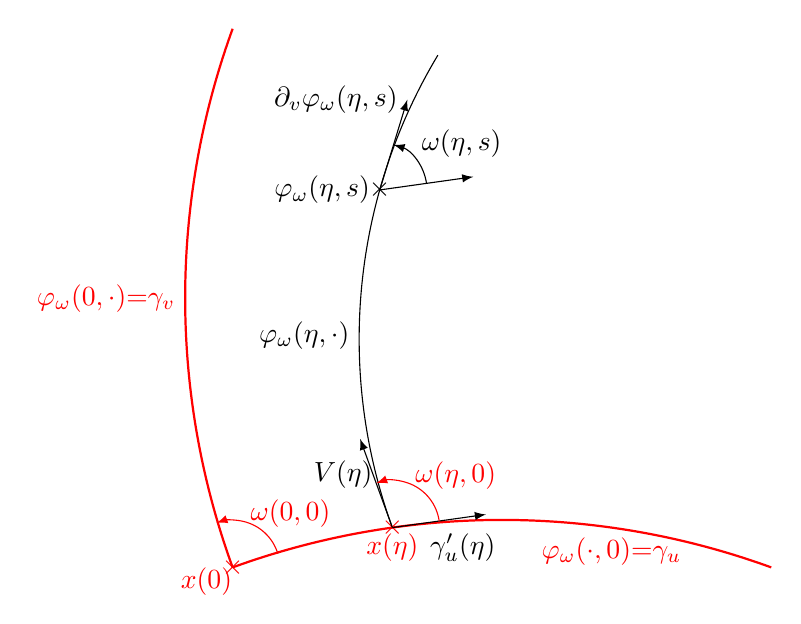
\begin{tikzpicture}[x=2cm,y=2cm]
    \draw[red] (0,0) node[anchor=north east,inner sep=0pt]{$x(0)$};
    \draw[red] (0,0) node{$\times$};
    \draw[thick,red] (0,0) arc[start angle=110,delta angle=-40,radius=5] coordinate[pos=0.7] (v1) coordinate[pos=0.3] (v2);
    \draw[red] (v1) node[anchor=north]{$\varphi_\omega(\cdot,0){=}\gamma_{u}$};
    \draw[thick,red] (0,0) arc[start angle=200,delta angle=-40,radius=5] coordinate[pos=0.5] (v3);
    \draw[red] (v3) node[anchor=east]{$\varphi_\omega(0,\cdot){=}\gamma_{v}$};
    \draw (v2) arc[start angle=200,delta angle=-51,radius=3.5] coordinate[pos=0.4] (v4)  coordinate[pos=0.7] (v5);
    \draw (v4) node[anchor=east]{$\varphi_\omega(\eta,\cdot)$};
    \draw[red] (v2) node[anchor=north,inner sep=2pt]{$x(\eta)$};
    \draw[red] (v2) node{$\times$};
    \draw[-latex] (v2) -- ($(v2)+(8:.6)$) node[anchor=north west,pos=.3]{$\gamma_u'(\eta)$};
    \draw[-latex] (v2) -- ($(v2)+(110:.6)$) node[anchor=east, inner sep=0pt,pos=.6]{$V(\eta)$};
    \draw[-latex,red] ($(v2)+(8:0.3)$) arc[start angle=8,delta angle=102,radius=0.3];
    \draw[red] ($(v2)+(65:0.2)$) node[anchor=south west]{$\omega(\eta,0)$};
    \draw[red] ($(75:0.2)$) node[anchor=south west]{$\omega(0,0)$};
    \draw (v5) node[anchor=east]{$\varphi_\omega(\eta,s)$};
    \draw (v5) node{$\times$};
    \draw[-latex] (v5) -- ($(v5)+(73:.6)$) node[anchor=east]{$\partial_v\varphi_\omega(\eta,s)$};
    \draw[-latex] (v5) -- ($(v5)+(8:.6)$);
    \draw[-latex] ($(v5)+(8:0.3)$) arc[start angle=8,delta angle=65,radius=0.3];
    \draw ($(v5)+(35:0.25)$) node[anchor=south west]{$\omega(\eta,s)$};
    \draw[-latex,red] ($(17:0.3)$) arc[start angle=17,delta angle=93,radius=0.3];
  \end{tikzpicture}
  \caption{Illustration of the construction of the parametrization $\varphi_\omega$}\label{fig:construction2}
\end{figure}

\begin{proposition}[Continuity of the construction]\label{prop:cont-I}
Let $\surf$ be a smooth, open, complete, and simply connected surface, let $k,r\in\EN$, and let $D=[0,L_u]\Times[0,L_v]$, with $L_u,L_v\in\R^+_\ast$. For all $\gamma=(\gamma_u,\gamma_v)\in\Gamma^{r+2}([0,L_u])\Times\Gamma^{k+2}([0,L_v])$, the mapping $\I(\gamma,\cdot)$ is well defined. Moreover, let \sloppy $\gamma_1,\gamma_2\in\Gamma^{r+2}([0,L_u])\Times\Gamma^{k+2}([0,L_v])$, with $\gamma_1=(\gamma_{u,1}, \gamma_{v,1})$ and $\gamma_2=(\gamma_{u,2}, \gamma_{v,2})$, be such that $\gamma_{u,1}(0)=\gamma_{u,2}(0) = \gamma_{v,1}(0)=\gamma_{v,2}(0)$ and such that $\gamma_{u,1}'(0)=\gamma_{u,2}'(0)$ and $\gamma_{v,1}'(0)=\gamma_{v,2}'(0)$. Consider the two angle distributions $\omega_m\in \Theta^{r+1,k+1}_{\gamma_m}(D)$, for $m\in\{1,2\}$. Then, we have
\begin{equation}\label{eq:contr-I}
  \|\I(\gamma_m,\omega_m)\|_{\Phi^{r+1,k+2}(D)} \leq C%\left(\|\gamma_{u,m}\|_{\Gamma^{r+1}([0,L_u])},\|\omega_m\|_{\Theta^{r+1,k+1}(D)}\right), \text { if } r>0,
\end{equation}
where the constant $C$ depends on $L_u$, $L_v$, $\|\gamma_{u,m}\|_{\Gamma^{s}([0,L_u])}$, and $\|\omega_m\|_{\Theta^{r+1,k+1}(D)}$, with $s=\max(r+1,2)$.
Moreover, for all $L\in(0,L_v]$, setting $D_L=[0,L_u]\Times[0,L]$, we have
\small
\begin{subequations}\label{eq:cont-I}
\begin{align}\label{eq:cont-I1}
\begin{split}
  \|\I(\gamma_1,\omega_1) - \I(\gamma_2,\omega_2)\|_{\Phi^{0}(D_L)} &\leq ~C\Big(L\|\omega_1 - \omega_2\|_{\Theta^{1}(D_L)}\\
 &\qquad~+ \|\gamma_{u,2}-\gamma_{u,1}\|_{\Gamma^{2}([0,L_u])}\Big),
\end{split} \text{ if $r=0$ and $k=0$},\\\label{eq:cont-I2}
\begin{split}
  \|\I(\gamma_1,\omega_1) - \I(\gamma_2,\omega_2)\|_{\Phi^{1,k+2}(D_L)} &\leq C\Big(\|\omega_1 - \omega_2\|_{\Theta^{1,k+1}(D_L)}\\
 &\qquad~+ \|\gamma_{u,2}-\gamma_{u,1}\|_{\Gamma^{2}([0,L_u])}\Big),
\end{split}~~ \text{ if } r=0,\\\label{eq:cont-I3}
\begin{split}
  \|\I(\gamma_1,\omega_1) - \I(\gamma_2,\omega_2)\|_{\Phi^{r+1,k+2}(D_L)} &\leq C\Big(\|\omega_1 - \omega_2\|_{\Theta^{r+1,k+1}(D_L)}\\
 &\qquad~+ \|\gamma_{u,2}-\gamma_{u,1}\|_{\Gamma^{r+1}([0,L_u])}\Big),
\end{split} ~~\text{ if } r>0,
\end{align}
\end{subequations}
\normalsize
where the constant $C$ depends on $L_u$, $L_v$, $\|\gamma_{u,i}\|_{\Gamma^{s}([0,L_u])}$, and $\|\omega_i\|_{\Theta^{r+1,k+1}(D)}$, with $i\in\{1,2\}$ and $s=\max(r+1,2)$.
\end{proposition}
\begin{proof}
  Since the construction of the mapping $\varphi_\omega$ is the same as that in the construction of Proposition \ref{prop:constr-courbe}, we only need to prove that the boundary conditions used in the construction of $\varphi_\omega$ are smooth enough. %To prove the claim, we only need to show that The mapping $\varphi$ is well defined by Proposition \ref{prop:constr-courbe} and we have $\varphi\in\Phi^{r,k+2}$ by the same proposition.
% be two curves of respective geodesic curvatures $\ko_{u,1}:[0,L_u]\to\R$ and $\ko_{u,2}:[0,L_v]\to\R$
  We denote $\ko_{u,1}:[0,L_u]\to\R$ and $\ko_{u,2}:[0,L_v]\to\R$ the geodesic curvatures of the curves $\gamma_{u,1}$ and $\gamma_{u,2}$ respectively.
  Using the notation of Proposition \ref{prop:constr-courbe}, for all $m\in\{1,2\}$ and $u\in[0,L_u]$, we set $x_m(u) = \gamma_{u,m}(u)$ and 
  \begin{equation}\label{eq:pr-cont-constr}
    V_m(u) = \RR_{\gamma_{u,m}(u)}(\omega_m(u,0))\gamma_{u,m}'(u) = \cos(\omega_m(u,0))\gamma_{u,m}'(u) + \sin(\omega_m(u,0))\gamma_{u,m}^{\prime\perp}(u),
  \end{equation}
 where $\gamma_{u,m}^{\prime\perp}$ is the direct $\frac{\pi}{2}$-rotation of $\gamma_{u,m}'$.  % and, owing to Proposition \ref{prop:constr-courbe}, we obtain
  % \begin{equation*}
  %   \sigma_m(u,\cdot) := \sigma(\gamma_{u,m},\gamma_{v,m},\omega_m(u,\cdot))\in \Gamma^{k}_{L_v}.
  % \end{equation*}
 Since $|V_m|_g=1$, we infer from \eqref{eq:equiv} that $\|V_m\|_{C^0([0,L_u])}\leq \Csurf$, for all $m\in\{1,2\}$. Furthermore, using that $\omega_1\in\Theta^{r+1,k+1}_{\gamma_1}(D)$ and  $\omega_2\in \Theta^{r+1,k+1}_{\gamma_2}(D)$ both satisfy the boundary conditions \eqref{eq:cond-bord-angle}, we obtain
 \begin{equation*}
   |\omega_2-\omega_1|(u,0) = \Big|\int_0^u\ko_{u,2}-\int_0^u\ko_{u,1}\Big| \leq \int_0^u|\ko_{u,2}-\ko_{u,1}|.
 \end{equation*}
 Hence, using \eqref{eq:pr-cont-constr}, we obtain by a straightforward computation that
 % \begin{equation*}
 %   \|\omega_2(\cdot,0)-\omega_1(\cdot,0)\|_{L^p([0,L_u])} \lesssim \|\ko_2-\ko_1\|_{L^p([0,L_u])},
 % \end{equation*}
 % so that we have, using \eqref{eq:pr-cont-constr},
 \begin{equation}\label{eq:pr-cont-constr2}
   \|V_2-V_1\|_{C^0([0,L_u])} \leq C\Big( \|\ko_{u,2}-\ko_{u,1}\|_{C^0([0,L_u])} + \|\gamma_2'-\gamma_1'\|_{C^0([0,L_u])}\Big).
 \end{equation}
 Let $m\in\{1,2\}$. Since $\omega_m$ satisfies the boundary conditions \eqref{eq:cond-bord-angle} given by the arc-length parametrized curve $\gamma_{u,m}$, we infer from the definition of geodesic curvature \eqref{eq:geod-dual1} that
  \begin{align*}
   \frac{D}{du}\gamma_{u,m}^\prime =\ko_{u,m}\gamma_{u,m}^{\prime\perp}= -\DU\omega_m(\cdot,0)\gamma_{u,m}^{\prime\perp},\\ 
   \frac{D}{du}\gamma_{u,m}^{\prime\perp} =-\ko_{u,m}\gamma_{u,m}^{\prime}= \DU\omega_m(\cdot,0)\gamma_{u,m}^{\prime},
  \end{align*}
  where $\frac{D}{du}$ is the covariant derivative along the curve $\gamma_{u,m}$. Hence, we deduce from \eqref{eq:pr-cont-constr} that
\begin{align*}
  \frac{D}{du}V_m(u) &=~~ \partial_u\omega_m(u,0)\left(\cos(\omega_m(u,0))\gamma_{u,m}^{\prime\perp} - \sin(\omega_m(u,0))\gamma_{u,m}'\right) \\
&\quad+ \cos(\omega_m(u,0))\frac{D}{du}\gamma_{u,m}^\prime + \sin(\omega_m(u,0))\frac{D}{du}\gamma_{u,m}^{\prime\perp}= 0,\snum\label{eq:pr-cont-constr2bis}
\end{align*}
for all $u\in[0,L_u]$. Therefore, in the same manner as in Proposition \ref{prop:constr-courbe}, using that $V_m$ is bounded, \eqref{eq:pr-cont-constr2} and \eqref{eq:pr-cont-constr2bis}, we obtain 
 \begin{equation}\label{eq:pr-cont-constr3bis}
\|V_m\|_{C^{r+1}([0,L_u])}\leq C,\quad\|V_1-V_2\|_{C^{r+1}([0,L_u])}\leq \tilde C\|\gamma_{u,1}-\gamma_{u,2}\|_{\Gamma^s([0,L_u])},
\end{equation}
where $s=\max(r+1,2)$, the constant $C$ depends on $L_u$, $L_v$, and $\|\gamma_{u,m}\|_{\Gamma^{s}([0,L_u])}$, and the constant $\tilde C$ depends on $L_u$, $L_v$, and $\|\gamma_{u,l}\|_{\Gamma^{s}([0,L_u])}$, with $l\in\{1,2\}$.
Moreover, since $x_m=\gamma_{u,m}$, we have%Using Proposition \ref{prop:constr-courbe} on curves $\gamma_{u,1}$ and $\gamma_{u,2}$, we obtain 
\begin{equation}\label{eq:pr-cont-constr3}
\|x_m\|_{C^{r+1}([0,L_u])}= \|\gamma_{u,m}\|_{\Gamma^{r+1}([0,L_u])},\quad\|x_1-x_2\|_{C^{r+1}([0,L_u])}= \|\gamma_{u,1}-\gamma_{u,2}\|_{\Gamma^{r+1}([0,L_u])}.
\end{equation}
We set $\kop_{v,m}(u,\cdot) := \partial_v\omega_m(u,\cdot):[0,L_v]\to\R$, for all $u\in[0,L_u]$.
 We conclude the proof using \eqref{eq:pr-cont-constr3bis}, \eqref{eq:pr-cont-constr3} and Proposition \ref{prop:constr-courbe} with regularity $(r{+}1,k)$, i.e., with $x_1,x_2\in C^{r+1}([0,L_u])$, $V_1,V_2\in C^{r+1}([0,L_u])$ and $\kop_{v,1},\kop_{v,2}\in C^{r+1}([0,L_u],C^{k}([0,L_v]))$.
\end{proof}

\subsection{Regularity of the candidate Chebyshev nets}\label{sec:reg-candidate}
Let us now consider the case where we have the same regularity in both coordinates in the data permitting the construction of $\varphi_\omega$, i.e., $r=k$. Then, taking $r=k$ in Proposition \ref{prop:cont-I} gives an optimal estimate in the second coordinate regularity but a suboptimal estimate in the first coordinate, since we expect $C^{k+2}$-regularity in both directions.
We show in this section that, whenever the mapping constructed satisfies the integrability equation \eqref{eq:cond-integr}, 
it has indeed the expected regularity in the first variable as well.
\begin{proposition}[Regularity of mappings satisfying the integrability condition]\label{prop:reg-cheb}
  Keeping the assumptions of Proposition \ref{prop:cont-I} with $k=r\in\EN$, we moreover suppose that $\omega_m\in\Theta^{k+1}(D)$ satisfies the Hazzidakis formula \eqref{eq:hazz-form} with $\varphi_m:=\I(\gamma_m,\omega_m)$, i.e.,
  \begin{equation}\label{eq:hazz-form-bis}
    \begin{split}
  \omega_m(u,v) = &~\angle\big(\gamma_{u,m}'(0),\gamma_{v,m}'(0)\big) - \int_0^u\ko_{u,m} + \int_{0}^v\ko_{v,m}\\
  & -\int_{0}^{u} \int_{0}^{v} K\big[\I(\gamma_m,\omega_m)(t,s)\big]\sin(\omega_m(t,s)) \dt \ds,
  \end{split}
  \end{equation}
  for all $m\in\{1,2\}$. Then, we have $\varphi_m \in \Phi^{k+2}(D)$ and
\begin{equation}
\label{eq:borne-cheb}
 \|\I(\gamma_m,\omega_m)\|_{\Phi^{k+2}(D)} \leq C,
\end{equation}
where the constant $C$ depends on $L_u$, $L_v$, $\|\gamma_{u,m}\|_{\Gamma^{k+2}([0,L_u])}$, and $\|\omega_m\|_{\Theta^{k+1}(D)}$, for all $m\in\{1,2\}$. Moreover, we have
\begin{equation}\label{eq:reg-cheb}
\begin{split}
\|\I(\gamma_1,\omega_1) - \I(\gamma_2,\omega_2)\|_{\Phi^{k+2}(D)} \leq C\Big(&\|\omega_1 - \omega_2\|_{\Theta^{k+1}(D)} \\
& + \|\gamma_{2,u}-\gamma_{1,u}\|_{\Gamma^{k+2}([0,L_u])}\Big)
\end{split}
\end{equation}
where the constant $C$ depends on $L_u$, $L_v$, $\|\gamma_{u,i}\|_{\Gamma^{k+2}([0,L_u])}$ and $\|\omega_i\|_{\Theta^{k+1}(D)}$, for $i\in\{1,2\}$.
\end{proposition}

\begin{proof}
  Let $m\in\{1,2\}$. First, owing to Proposition \ref{prop:cont-I}, we have $\varphi_m = \I(\gamma_{m},\omega_m)\in \Phi^{k+1,k+2}(D)$. We denote $\kop_{v,m}=\partial_v\omega_m\in C^{k+1}([0,L_u],C^{k}([0,L_v]))$ the geodesic curvatures of the $v$-coordinate curves of $\varphi_m$.
  Let us remark that, since $\omega_m\in\Theta^{1}(D)$ satisfies the Hazzidakis formula \eqref{eq:hazz-form-bis}, $\omega_m$ satisfies the integrability condition  \eqref{eq:cond-integr}, i.e.,
\begin{equation}\label{eq:cond-integr2}
  \DUV \omega_m = -K(\varphi_m) \sin(\omega_m).
\end{equation}
Then, the claim is obtained by remarking that \eqref{eq:cond-integr2} implies that the geodesic curvatures $\kop_{v,m}$ of the $v$-coordinate curves satisfy
\begin{equation}\label{eq:pr-smooth1}
  \kop_{v,m}\in C^{k+2}([0,L_u],C^{k}([0,L_v])).
\end{equation}
Indeed, for all $i,j\in\{0,...,k\}$, we have
\begin{equation}\label{eq:pr-smooth2}
\partial_u^{i+1}\partial_v^j\kop_{v,m} = \partial_u^{i}\partial_v^{j}\big(\DU\DV\omega_m\big) = \partial_u^{i}\partial_v^{j}\Big({-}K(\varphi_m) \sin(\omega_m)\Big).
\end{equation}
Hence, since $\omega_m\in \Theta_{\gamma_m}^{k+1}(D)$ and $\varphi_m\in \Phi^{k+1,k+2}(D)$ and since $K$ is smooth, we infer that \eqref{eq:pr-smooth1} holds and that \eqref{eq:pr-smooth2} is satisfied for all $i\in\{0,...,k{+}1\}$ and $j\in\{0,...,k\}$. Furthermore, we have
\begin{equation}\label{eq:pr-smooth3}
    \DU^2\kop_{v,m}=\DU\big({-}K(\varphi_m) \sin(\omega_m)\big)= -\sin(\omega_m)\nabla K(\varphi_m)\partial_u\varphi_m-K(\varphi_m)\cos(\omega_m)\partial_u\omega_m,
\end{equation}
so that we easily obtain $\big\|\DU^2\kop_{v,m}\big\|_{C^{k}([0,L_u],C^k([0,L_v]))}\leq C$, where the constant $C$ depends on $L_u$, $L_v$, $\|\omega_m\|_{\Theta^{k+1}(D)}$, and $\|\varphi_m\|_{\Phi^{k+1}(D)}$. Using moreover \eqref{eq:contr-I}, we conclude that the constant $C$ only depends on $L_u$, $L_v$,  $\|\omega_m\|_{\Theta^{k+1}(D)}$, and $\|\gamma_{u,m}\|_{\Gamma^{s}([0,L_u])}$, with $s=\max(k+1,2)$. We infer that
\begin{equation}\label{eq:pr-smooth4}
    \big\|\kop_{v,m}\big\|_{C^{k+2}([0,L_u],C^{k}([0,L_v]))}\leq C,
  \end{equation}where the constant $C$ depends on $L_u$, $L_v$, $\|\omega_m\|_{\Theta^{k+1}(D)}$, and $\|\gamma_{u,m}\|_{\Gamma^{s}([0,L_u])}$.
  Recalling that $s=\max(k+1,2)$, we deduce from \eqref{eq:pr-smooth3} and \eqref{eq:cont-I} that
\begin{align*}
      \big\|\DU^2\kop_{v,2}-\DU^2\kop_{v,1}\big\|_{C^{k}([0,L_u],C^{k}([0,L_v]))} &\leq \tilde C\Big(\|\omega_2-\omega_1\|_{\Theta^{k+1}(D)} +\|\varphi_2-\varphi_1\|_{\Phi^{k+1}(D)}\Big)\\
      &\leq C\Big(\|\omega_2-\omega_1\|_{\Theta^{k+1}(D)} + \|\gamma_{u,2}-\gamma_{u,1}\|_{\Gamma^{s}([0,L_u])}\Big),
\end{align*}
where the constants $C,\tilde C$ depend on $L_u$, $L_v$, $\|\gamma_{u,i}\|_{\Gamma^{s}([0,L_u])}$, and $\|\omega_i\|_{\Theta^{k+1}(D)}$, with $i\in\{1,2\}$. We conclude that 
\begin{equation}\label{eq:pr-smooth5}
      \big\|\kop_{v,2}-\kop_{v,1}\big\|_{C^{k+2}([0,L_u],C^{k}([0,L_v]))} \leq C\Big(\|\omega_2-\omega_1\|_{\Theta^{k+1}(D)} + \|\gamma_{u,2}-\gamma_{u,1}\|_{\Gamma^{s}([0,L_u])}\Big),
    \end{equation}
 where the constant $C$ depends on $L_u$, $L_v$, $\|\gamma_{u,i}\|_{\Gamma^{s}([0,L_u])}$, and $\|\omega_i\|_{\Theta^{k+1}(D)}$, with $i\in\{1,2\}$.   
   As in the proof of Proposition \ref{prop:cont-I}, for all $u\in[0,L_u]$, we set $x_m(u) = \gamma_{u,m}(u)$ and
  \begin{equation*}
    V_m(u) = \RR_{\gamma_{u,m}(u)}(\omega_m(u,0))\gamma_{u,m}'(u).
  \end{equation*} 
Before we apply Proposition \ref{prop:constr-courbe} with regularity $(k+2,k)$, let us first note that, as in the proof of Proposition \ref{prop:cont-I}, the estimate on $x_1,x_2\in C^{k+2}([0,L_u])$, $V_1,V_2\in C^{k+2}([0,L_u])$ is given by \eqref{eq:pr-cont-constr3bis}, \eqref{eq:pr-cont-constr3}. Hence, the claim follows from the estimate on $\kop_{v,1},\kop_{v,2}\in C^{k+2}([0,L_u],C^k([0,L_v]))$ given by \eqref{eq:pr-smooth4} and \eqref{eq:pr-smooth5}, and Proposition \ref{prop:constr-courbe} with regularity $(k+2,k)$.
\end{proof}

\subsection{From integrability conditions to Chebyshev nets}\label{sec:reg-cheb}
\begin{proposition}[From integrability conditions to Chebyshev nets]\label{prop:cheb}
Let $\surf$ be a smooth, open, complete, and simply connected surface, let $D = [0,L_u]\times[0,L_v]$, with $L_u,L_v\in\R^+_\ast$, and let $k\geq 1$. Let $\gamma=(\gamma_u,\gamma_v)\in\Gamma^{k+2}([0,L_u])\Times\Gamma^{k+2}([0,L_v])$. Assume that $\omega\in\Theta^{k+1}_{\gamma}(D)$ is an angle distribution satisfying the integrability condition \eqref{eq:cond-integr}, with $\varphi:=\I(\gamma,\omega)\in\Phi^{k+2}(D)$. Suppose moreover that $0<\omega(u,v)<\pi$, for all $(u,v)\in D$. Then, the mapping $\varphi$ is a Chebyshev net in the sense that it satisfies \eqref{eq:cheb-def-c3}.
\end{proposition}

\begin{proof}
  First, owing to Proposition \ref{prop:reg-cheb}, we have that $\varphi\in \Phi^{k+2}(D)$, so that $\varphi$ has $C^3$-regularity.
  % First, recall that we have, by definition, 
% \begin{equation}
% \partial_u \varphi(u,v) = \partial_u\sigma_u(v), \quad\partial_v \varphi(u,v) = \sigma_u'(v),\quad \forall(u,v)\in [0,L_u]\Times[0,L_v].
% \end{equation}
  %We set $\partial_u := \partial_u \varphi$ and $\partial_v := \partial_v\varphi$.
  Since the $v$-coordinate curves are arc-length parametrized curves, we have by construction $|\PV|_g(u,v) = 1$, and we set $R(u,v) = |\PU|_g(u,v)$, for all $(u,v)\in D$. Then, since $\gamma_u$ is an arc-length parametrized curve, we have $R(u,0) = 1$, for all $u\in [0,L_u]$. The proof amounts to showing that
\begin{equation}
\label{eq:pr-R}
 \exists L\in(0,L_v],\quad \partial_v R(u,v) = 0, \quad\forall (u,v)\in [0,L_u]\Times[0,L].
\end{equation}
Indeed, suppose that \eqref{eq:pr-R} is satisfied and denote $I\subset [0,L_v]$ the maximal interval on which we have $R(u,v) = 1$, for all $(u,v)\in [0,L_u]\Times I$. Owing to \eqref{eq:pr-R}, we first have that $[0,L]\subset I$, so that $I$ is nonempty. Moreover, suppose that $[0,\tilde L_0]\subset I$, for some $\tilde L_0\in(0,L_v]$. Then, since the angle distribution $\omega\big|_{[0,L_u]\Times[\tilde L_0,L_v]}$ and the mapping $\varphi\big|_{[0,L_u]\Times[\tilde L_0,L_v]}$ satisfy the hypotheses of the proposition, we infer from \eqref{eq:pr-R} that there exists $\tilde L_1\in(\tilde L_0,L_v]$ such that $[0,\tilde L_1]\subset I$. Hence, $I$ is open in $[0,L_v]$, and we deduce from the continuity of $R$ that $I$ is closed. Therefore, \eqref{eq:pr-R} implies the claim.
%Therefore, the proof consists in computing the Gaussian curvature $K$ associated with the parametrization $\varphi$
% in the basis $(\partial_u \varphi,\partial_v\varphi)$ of the tangent plane 
%and in deducing \eqref{eq:pr-R} by identification with \eqref{eq:cond-integr}.

%We use in the rest of the proof the usual differential geometry notation: $f_u = \partial_u f$ and $f_v = \partial_v f$, for any $C^1$-function $f$.
We now suppose that $L\in (0,L_v]$ is small enough so that $R(u,v)>0$, for all $(u,v)\in[0,L_u]\Times[0, L]$, we set $D_L=[0,L_u]\Times[0,L]$, and we set $X_1(u,v) := \big\langle \NPU(u,v), \PV(u,v)\big\rangle_g$ and \sloppy $X_2(u,v) := \big\langle\frac{\PU^\perp}{R}(u,v), \PV(u,v)\big\rangle_g$, for all $(u,v)\in D_L$. Note that by definition $X_1^2+X_2^2=1$ in $D_L$. 
Recalling that $R(\cdot,0)=1$ by construction of $\varphi$, we have
\begin{subequations}\label{eq:cond-bord-X}
  \begin{align}\label{eq:cond-bord-X1}
  X_1(u,0)&=\big\langle\PU,\PV\big\rangle_g(u,0)=\cos\big(\omega(u,0)\big),\\\label{eq:cond-bord-X2}
  X_2(u,0)&=\big\langle\PU^\perp,\PV\big\rangle_g(u,0)=\sin\big(\omega(u,0)\big),
  \end{align}
  \end{subequations}
for all $u\in[0,L_u]$. Hence, since $X_2$ is continuous, up to reducing $L$, we have $X_2>0$ due to the assumption that $0<\omega<\pi$. 
%, and, by construction, we have $\langle\partial_u,\partial_v\rangle(u,0) = \cos(\omega(u,0))$, for all $u\in [0,L_u]$

We prove \eqref{eq:pr-R} as follows. We show that an identification of the Gaussian curvature computed using the local coordinates $\varphi$ with \eqref{eq:cond-integr} leads to the following integro-differential equation on $R$ in the $v$-coordinates:
\begin{equation}\label{eq:int-diff-eq0}
\DVV R =\DV\omega \DV RT  + \frac{(\DV R)^2}{R}T^2 -K(\varphi)X_2\Big(\sin\omega\int_0^v\frac{\DV R}{X_2}\sin\omega
+\cos\omega\int_0^v\frac{\DV R}{X_2}\cos\omega\Big),
\end{equation}
with $T = \displaystyle\frac{X_1}{X_2}$. We show that $\DV R=0$ is the unique solution to \eqref{eq:int-diff-eq0} to prove the claim \eqref{eq:pr-R}. First, we compute in Step \ref{step:bound-cond} the initial conditions satisfied by $\DV R$ necessary to obtain the uniqueness of the solution of \eqref{eq:int-diff-eq0}, i.e., we prove that $\DV R(\cdot,0)=0$. Then, we compute in Steps \ref{step:gauss-curv1}-\ref{step:gauss-curv3} the Gaussian curvature $K$ in terms of $R$, $X_1$ and $X_2$. Using \eqref{eq:cond-integr}, we reduce the Gaussian curvature to \eqref{eq:int-diff-eq0} in Step \ref{step:bound-sec-mem} and we conclude in Step \ref{step:concl}.

\begin{proofpart}[Initial conditions]\label{step:bound-cond}
  We prove that $\partial_v R(u,0) = 0$, for all $u\in[0,L_u]$.

We denote in what follows $D_{\DU} Y$ and $D_{\DV} Y$ the covariant derivative of the vector field $Y$ in the directions $\PU$ and $\PV$, respectively. First, since $R(\cdot,0)=1$, we have that $\DU R(u,0) = 0$, for all $u\in[0,L_u]$. Moreover, since $\omega$ satisfies the boundary conditions \eqref{eq:cond-bord-angle}, we have that $D_{\DU}\PU(u,0) = -[\DU\omega\PU^{\perp}](u,0)$. Combining these results with \eqref{eq:cond-bord-X}, we obtain 
\begin{align*}
\frac{1}{2}\DV(R^2)(u,0) &= \big\langle D_{\DV}\PU,\PU\big\rangle_g(u,0) 
= \partial_u(RX_1)(u,0) - \big\langle D_{\DU}\PU,\PV\big\rangle_g(u,0)\\
&= R(u,0)\DU X_{1}(u,0) + \big\langle \DU\omega \PU^\perp,\PV\big\rangle_g(u,0) \\
&= \frac{d}{du} [\cos(\omega(u,0))] + \DU\omega(u,0) \sin(\omega(u,0))=0,
\end{align*}
for all $u\in[0,L_u]$. Therefore, we have $\partial_v R(u,0) = 0$, for all $u\in[0,L_u]$.
\end{proofpart}
\begin{proofpart}[Computation of the Gaussian curvature ($1^{\text{st}}$ part)]\label{step:gauss-curv1}
We prove the following relations on the parallel transport of vectors:
\begin{subequations}\label{eq:pr-DU-dum}
  \begin{align}\label{eq:pr-DU1}
D_{\partial_u}\PU &= \left(\frac{\DU R}{R}+\frac{X_1}{X_2^2}(\DV R-\DU X_1)\right)\PU+\left(\frac{R}{X_2^2}(\DU X_1-\DV R)\right)\PV,\\\label{eq:pr-DU2}
D_{\partial_v}\PU = D_{\partial_u}\PV &= \frac{\DV R}{RX_2^2}\PU - \frac{\DV RX_1}{X_2^2}\PV,\\\label{eq:pr-DV1}
D_{\partial_v}\PV &= \DV\omega\PV^\perp.
\end{align}
\end{subequations}
The results \eqref{eq:pr-DU1} and \eqref{eq:pr-DU2} easily follow from the identities
\begin{align*}
  \big\langle D_{\partial_u}\PU,\PU\big\rangle_g &= R\DU R,\\
\big\langle D_{\partial_u}\PU,\PV\big\rangle_g &= \partial_u(RX_1) - \big\langle\PU,D_{\partial_v}\PU\big\rangle_g = \DU RX_1+R\DU X_{1}-R\DV R,\\
\big\langle D_{\partial_u}\PV,\PU\big\rangle_g &= R\DV R,\\\big\langle D_{\partial_u}\PV,\PV\big\rangle_g &= 0,
\end{align*}
where we have used in the last equality the fact that $|\PV|_g=1$. Equation \eqref{eq:pr-DV1} is obtained using that the $v$-coordinate curves of $\varphi$ are arc-length parametrized and have by construction a geodesic curvature given by $\DV\omega$.
\end{proofpart}
\begin{proofpart}[Computation of the Gaussian curvature ($2^{\text{nd}}$ part)]\label{step:gauss-curv2}
We prove that $X_1$ and $X_2$ satisfy
\begin{subequations}\label{eq:syst_angle1}
\begin{align}\label{eq:syst_angle1a}
\DV X_{1}&=-\DV\omega X_2 - \frac{\DV R}{R} X_1,\\
\DV X_{2} &=\DV\omega X_1 + \frac{X_1}{X_2} \frac{\DV R}{R}X_1.\label{eq:syst_angle1b}
\end{align}
\end{subequations}
First, using that $\langle D_{\partial_v}\PU,\PV\rangle = 0$ and \eqref{eq:pr-DV1}, we obtain 
\begin{align*}
  \partial_v X_1& = \big\langle D_{\partial_v}\PV,\NPU\big\rangle_g + \big\langle D_{\partial_v}\NPU,\PV\big\rangle_g  = \DV\omega \big\langle \PV^\perp,\NPU\big\rangle_g+ \langle-\frac{\DV R}{R^2}\PU+\frac{1}{R}D_{\partial_v}\PU,\PV\rangle_g\\
  &=  -\DV\omega X_2 - \frac{\DV R}{R} X_1,
\end{align*}
which proves \eqref{eq:syst_angle1a}.
% where $|\partial_v|_g=1$ implies that
% \[
% \langle D_{\partial_v}\partial_u,\partial_v\rangle = \langle D_{\partial_u}\partial_v,\partial_v\rangle = \frac{1}{2}\partial_u\langle\partial_v,\partial_v\rangle = 0 \text{ and } \langle D_{\partial_v}\partial_v,\partial_v\rangle = \frac{1}{2}\partial_v\langle\partial_v,\partial_v\rangle = 0.
% \]
Then, using that the geodesic curvatures of the $v$-coordinate curves of $\varphi$ is $\DV \omega$, we obtain $D_{\DV}\PV^\perp=-\DV\omega\PV$. Moreover, a straightforward comptation gives
\begin{equation*}
  \PV^\perp = -\frac{1}{RX_2}\PU+T\PV,\quad\big\langle\PU^\perp,\PV\big\rangle_g=-\big\langle\PU,\PV^\perp\big\rangle_g.
\end{equation*}
Combining these results, we infer that
\begin{align*}
    \partial_v X_2 &= -\big\langle D_{\partial_v}\NPU,\PV^\perp\big\rangle_g - \big\langle D_{\partial_v}\PV^\perp,\NPU\big\rangle_g \\
    &= \frac{\DV R}{R^2}\big\langle\PU,\PV^\perp\big\rangle_g - \frac{1}{R} \big\langle D_{\partial_u}\PV,\PV^\perp\big\rangle_g + \DV\omega\big\langle\PV,\NPU\big\rangle_g \\
                   &=-\frac{\DV R}{R}X_2-\frac{1}{R}\big\langle D_{\partial_u}\PV,-\frac{1}{RX_2}\PU+T\PV\big\rangle_g + \DV\omega X_1 \\
                   &= - \frac{\DV R}{R}X_2 +  \frac{\DV(R^2)}{2R^2X_2} + \DV\omega X_1 = \frac{\DV R}{R}\big(\frac{1}{X_2}-X_2\big)  + \DV\omega X_1\\
  &=\DV\omega X_1 + \frac{X_1}{X_2} \frac{\DV R}{R}X_1.
\end{align*}
\end{proofpart}


\begin{proofpart}[Computation of the Gaussian curvature ($3^{\text{rd}}$ part)]\label{step:gauss-curv3}
  We now compute the expression of the Gaussian curvature $K$ in the local parametrization $\varphi$. Note that the metric induced by $\varphi$ is $\tilde g = R^2du^2 + 2RX_1 dudv + dv^2$ giving $\det\tilde g = R^2X_2^2$. Then, recall that, by definition, the Gaussian curvature $K$ satisfies
\begin{equation}\label{eq:def-gauss-curv}
K\det \tilde g = \big\langle D_{\partial_v}D_{\partial_u}\PU - D_{\partial_u}D_{\partial_v}\PU,\PV\big\rangle_g.
\end{equation}
Using \eqref{eq:pr-DU1}, we first obtain that
\begin{align*}
  \big\langle D_{\partial_v}D_{\partial_u}\PU,\PV\big\rangle_g &= \big\langle D_{\partial_v}\big(A\PU+B\PV\big),\PV\big\rangle_g\\
  &=A \big\langle D_{\DV}\PU,\PV\big\rangle_g + B\langle D_{\DV}\PV,\PV\big\rangle_g + RX_1\DV A  + \DV B, 
\end{align*}
with $A=\frac{\DU R}{R}+\frac{X_1}{X_2^2}(\DV R-\DU X_{1})$ and $B = \frac{R}{X_2^2}(\DU X_{1}-\DV R)$. Then, we infer that
\small
\begin{align*}
 \big\langle D_{\partial_v}D_{\partial_u}\PU,\PV\big\rangle_g &= RX_1\DV A  + \DV B \\
 &= \DV\left(\frac{\DU R}{R}\right)RX_1
 +RX_1^2\DV\left(\frac{\DV R-\DU X_{1}}{X_2^2}\right) + RX_1\DV X_{1}\frac{\DV R-\DU X_{1}}{X_2^2}\\
 &\quad - \DV R\frac{\DV R-\DU X_{1}}{X_2^2}-R\DV\left(\frac{\DV R-\DU X_{1}}{X_2^2}\right)\\
                                                              &=\DV\left(\frac{\DU R}{R}\right)RX_1 -RX_2^2\DV\left(\frac{\DV R-\DU X_{1}}{X_2^2}\right) \\
  &\quad+ RX_1\DV X_{1}\frac{\DV R-\DU X_{1}}{X_2^2}- \DV R\frac{\DV R-\DU X_{1}}{X_2^2}.\snum\label{eq:pr-st-gauss3-1}
\end{align*}
\normalsize
Secondly, using \eqref{eq:pr-DU2}, we obtain that
\small
\begin{align*}
\big\langle D_{\partial_u}D_{\partial_v}\PU,\PV\big\rangle_g &= \big\langle D_{\partial_u}\left[\frac{\DV R}{RX_2^2}\PU - \frac{\DV RX_1}{X_2^2}\PV\right],\PV\big\rangle_g\\
&= \frac{\DV R}{RX_2^2}\big\langle D_{\partial_u}\PU,\PV\big\rangle_g - \frac{\DV RX_1}{X_2^2}\big\langle D_{\partial_u}\PV,\PV\big\rangle_g
+ RX_1\DU\left(\frac{\DV R}{RX_2^2}\right) - \DU\left(\frac{\DV RX_1}{X_2^2}\right)\\
&= \frac{\DV R}{RX_2^2}\big\langle D_{\partial_u}\PU,\PV\big\rangle_g  -\frac{\DU R}{R^2}\frac{\DV R}{X_2^2}RX_1 + \DU\left(\frac{\DV R}{X_2^2}\right)X_1- \DU\left(\frac{\DV R}{X_2^2}\right)X_1 - \frac{\DU X_{1}\DV R}{X_2^2}\\
&=\frac{\DV R}{X_2^2} \left(\frac{1}{R}\big\langle D_{\partial_u}\PU,\PV\big\rangle_g - \frac{X_1\DU R}{R}-\DU X_{1}\right).
\end{align*}
\normalsize
Since $\langle D_{\partial_u}\PU,\PV\rangle_g = \DU RX_1+R\DU X_{1}-R\DV R$, we infer that
\begin{equation}\label{eq:pr-st-gauss3-2}
  \big\langle D_{\partial_v}D_{\partial_u}\PU,\PV\big\rangle_g=-\frac{(\DV R)^2}{X_2^2}.
\end{equation}
Combining \eqref{eq:def-gauss-curv}, \eqref{eq:pr-st-gauss3-1} and \eqref{eq:pr-st-gauss3-2} gives
\small
\begin{align*}
K\det \tilde g &= -RX_2^2\DV\left(\frac{\DV R-\DU X_{1}}{X_2^2}\right) + RX_1\DV X_{1}\frac{\DV R-\DU X_{1}}{X_2^2} 
+ \frac{\DV R\DU X_{1}}{X_2^2}+\DV\left(\frac{\DU R}{R}\right)RX_1\\
               &= \frac{1}{X_2^2}\big[RX_1\DV X_{1}(\DV R-\DU X_{1}) + \DV R\DU X_{1}\big] -R\DVV R+R \DUV X_{1} \\
  &\quad+ 2\DV X_{2}\frac{R(\DV R-\DU X_{1})}{X_2} + \DV\left(\frac{\DU R}{R}\right)RX_1\\
               &=  \frac{1}{X_2^2}\left[-RX_1\Big(\DV\omega X_2+\frac{\DV R}{R}X_1\Big) (\DV R-\DU X_{1})+\DV R\DU X_{1}\right]-R\DVV R-R\DU\left[\DV \omega X_2+\frac{\DV R}{R}X_1\right]\\
&\quad +2\left(\DV\omega X_1+\frac{X_1^2\DV R}{RX_2}\right)\frac{R(\DV R-\DU X_{1})}{X_2}+\DV\left(\frac{\DU R}{R}\right)RX_1,
\end{align*}
\normalsize
using \eqref{eq:syst_angle1} for the last equality. Then, we split the computation in two parts. First, we have
\begin{align*}
C &:= \frac{1}{X_2^2}\left[-RX_1\Big(\DV\omega X_2+\frac{\DV R}{R}X_1\Big)(\DV R-\DU X_{1})+\DV R\DU X_{1}\right]\\
  &= \frac{1}{X_2^2}\Big[-R\DV\omega X_1X_2\DV R+RX_1X_2\DV\omega \DU X_{1}-X_1^2(\DV R)^2+X_1^2\DU X_{1}\DV R+\DV R\DU X_{1}\big]\\
  &=-R\DV R\DV\omega T + RT\DV\omega\DU X_{1}-T^2(\DV R)^2+T^2\DU X_{1}\DV R+\frac{\DV R\DU X_{1}}{X_2^2}.\snum\label{eq:pr-st-gauss3-3}
\end{align*}
Then, we obtain
\begin{align*}
  E &:= -R\DVV R- R\DU\left[\DV\omega X_2+\frac{\DV R}{R}X_1\right]\\
  &\quad+ 2\left(\DV\omega X_1+\frac{X_1^2\DV R}{RX_2}\right)\frac{R(\DV R-\DU X_{1})}{X_2}+\DV\left(\frac{\DU R}{R}\right)RX_1\\
    &=-R\DVV R-R\Big[\DUV\omega X_2 + \DV\omega\DU X_{2}+\DV\left(\frac{\DU R}{R}\right)X_1+\frac{\DV R}{R}\DU X_{1}\Big] \\
  &\quad+ 2\DV\omega TR\big(\DV R-\DU X_{1}\big)+2T^2\DV R\big(\DV R-\DU X_{1}\big) + \DV\left(\frac{\DU R}{R}\right)RX_{1}\\
    &= -R\DVV R-R\DUV\omega X_2 - R\DV\omega(\DU X_{2}+T\DU X_{1}) - \DV R \DU X_{1}(1+T^2) \\
  &\quad-T\DU X_{1}R\DV\omega-T^2\DV R\DU X_{1}+2T\DV R\DV\omega R+2T^2(\DV R)^2.
\end{align*}
Moreover, since $X_1^2+X_2^2 = 1$, we have $1+T^2 = \frac{1}{X_2^2}$ and $T\DU X_{1}+\DU X_{2} = 0$. We infer that
\begin{equation}\label{eq:pr-st-gauss3-4}
  \begin{split}
    E =& -R\DVV R-R\DUV\omega X_2 - \frac{\DV R\DU X_{1}}{X_2^2}-T\DU X_{1}R\DV\omega\\&-T^2\DV R\DU X_{1}+2T\DV R\DV\omega R+2T^2(\DV R)^2.
    \end{split}
\end{equation}
We obtain by combining \eqref{eq:pr-st-gauss3-3} and \eqref{eq:pr-st-gauss3-4} that
\begin{equation}\label{eq:pr-st-gauss3-5}
  K\det \tilde g = C+E= T^2(\DV R)^2-R\DUV\omega X_2  -R\DVV R+TR\DV R \DV\omega.
\end{equation}
Using that $\det \tilde g=X_2^2R^2$ and dividing by $R$, we finally obtain
\begin{equation}
\label{eq:pr-equ-curv}
-\DV\omega \DV RT  -\frac{(\DV R)^2}{R}T^2 + \DVV R = -X_2(\DUV\omega+KX_2R).
\end{equation}
\end{proofpart}
\begin{proofpart}[Bound on the right-hand side of the equation \eqref{eq:pr-equ-curv}] \label{step:bound-sec-mem}
By \eqref{eq:pr-equ-curv} and the integrability condition \eqref{eq:cond-integr}, we have
\begin{equation}\label{eq:pr-st-contr}
\DVV R = \DV\omega \DV RT  + \frac{(\DV R)^2}{R}T^2 + K(\varphi)X_2\big[\sin(\omega)-X_2R\big].
\end{equation}
The proof is now reduced to showing that $\DV R=0$ is the unique solution to \eqref{eq:pr-st-contr} such that $\DV R(\cdot,0)=0$. To this end, we bound the right-hand side of this equation. Let $F_1 = \sin(\omega)-RX_2$ and $F_2 = \cos(\omega)-RX_1$. We infer from \eqref{eq:syst_angle1b} that
\begin{align*}
\DV F_{1} &= \DV \omega\cos(\omega) - \DV RX_2 - R\DV X_{2}= \DV\omega\big(\cos(\omega) - RX_1\big) - \DV R\big(X_2+TX_1\big)\\
&=\DV\omega F_2-\frac{\DV R}{X_2},
\end{align*}
using that $X_2+TX_1=X_2+\frac{1-X_2^2}{X_2}=\frac{1}{X_2}$ in the last equality. In the same manner, we deduce from \eqref{eq:syst_angle1a} that $\DV F_{2} = -\DV\omega F_1$, so that the couple $(F_1,F_2)$ satisfies the system of differential equations
\begin{equation*}
\left\{
\begin{split}
\DV F_{1}&=\DV\omega F_2 -\frac{\DV R}{X_2},\\
\DV F_{2} &=-\DV\omega F_1,
\end{split}
\right.
\end{equation*}
with $F_1(0) = F_2(0) = 0$, since $R(u,0) = 1$, $X_1(u,0) = \cos\omega(u,0)$, and $X_2(u,0) = \sin\omega(u,0)$, for all $u\in[0,L_1]$. A straightforward computation shows that the unique solution to this linear ordinary differential equation is 
\begin{subequations}\label{eq:ode}
\begin{align}\label{eq:ode1}
\begin{split}
(\sin \omega - X_2R)(u,v) = F_1(u,v) =&  -\sin\omega(u,v)\int_0^v\frac{\DV R}{X_2}(u,s)\sin\omega(u,s)\ds\\
&-\cos\omega(u,v)\int_0^v\frac{\DV R}{X_2}(u,s)\cos\omega(u,s)\ds,
\end{split}\\\label{eq:ode2}
\begin{split}
(\cos \omega - X_1R)(u,v) = F_2(u,v) =& -\cos \omega(u,v)\int_0^v\frac{\DV R}{X_2}(u,s)\sin\omega(u,s)\ds\\
&+\sin\omega(u,v)\int_0^v\frac{\DV R}{X_2}(u,s)\cos\omega(u,s)\ds,
\end{split}
\end{align}
\end{subequations}
since $\DV R(u,0) = 0$, for all $u\in[0,L_u]$, by Step \ref{step:bound-cond}.
\end{proofpart}
\begin{proofpart}[Conclusion]\label{step:concl}
Finally, we infer from \eqref{eq:pr-st-contr} and \eqref{eq:ode1} that
\begin{equation}\label{eq:int-diff-eq}
\DVV R =\DV\omega\DV RT  + \frac{(\DV R)^2}{R}T^2 -K(\varphi)X_2\Big(\sin\omega\int_0^v\frac{\DV R}{X_2}\sin\omega
+\cos\omega\int_0^v\frac{\DV R}{X_2}\cos\omega\Big).
\end{equation}
% Suppose that there exist two solutions $R$ and $\tilde R$ satisfying this equation and set $Z(t) = \DV R(u,t)-\DV\tilde R(u,t)$, for all $u\in [0,L_u]$ and $t\in[0,L]$.
Then, since $0<\omega(u,v)<\pi$, for all $(u,v)\in D_L$, we have that $T$ and $\frac{1}{X_2}$ are bounded. Using moreover that $\frac{1}{R}$, $\DV\omega$ and $K\circ\varphi$ are bounded, and using $\DV R(\cdot,0) = 0$, we infer from \eqref{eq:int-diff-eq} that
\begin{align*}
|\DV R(t)| &\leq \tilde C\Big( \int_0^t|\DV R(s)|\ds + \int_0^t|(\DV R)^2(s)|\ds + \int_0^t\int_0^s|\DV R(l)|\dl \ds\Big)\\
&\leq C\int_0^t|\DV R(s)|\ds,
\end{align*}
for all $u\in[0,L_u]$ and $t\in[0,L]$. Using Grönwall's inequality, we conclude that $\DV R(u,v) = 0$, for all $(u,v)\in D_L$. The claim follows.
\end{proofpart}
\end{proof}

\section{Existence and uniqueness of angle distribution}\label{subsec:exist-pt-fixe}
Let $k\in\EN$, let $D=[0,L_u]\Times[0,L_v]$, with $L_u,L_v\in\R^+_\ast$, and let $\gamma=(\gamma_u,\gamma_v)\in\Gamma^{k+2}([0,L_u])\Times\Gamma^{k+2}([0,L_v])$ be two curves of geodesic curvatures $\ko_u\in C^k([0,L_u],\R)$ and $\ko_v\in C^k([0,L_v],\R)$, respectively. In this section, we consider the Hazzidakis formula \eqref{eq:hazz-form} as an equation on $\omega\in\Theta^{k+1}_{\gamma}(D)$, i.e., on angle distributions satisfying the boundary conditions \eqref{eq:cond-bord-angle}. Hence, we define the mapping $F:\Theta_\gamma^{k+1}(D)\to\Theta^{k+1}_{\gamma}(D)$ by 
\begin{equation*} 
    F[\omega](u,v) = \angle\big(\gamma_u'(0),\gamma_v'(0)\big) - \int_0^u\ko_u + \int_{0}^v\ko_v -\int_{0}^{u} \int_{0}^{v} K\big[\I(\gamma,\omega)(t,s)\big]\sin(\omega(t,s)) \dt \ds,
\end{equation*}
and we prove in what follows that there exists a unique solution to 
\begin{equation} \label{eq:hazz2}
  \begin{split}
    \omega(u,v) = F[\omega](u,v),
    \end{split}
\end{equation}
for all $(u,v)\in D$. We first show in Subsection \ref{subsubsec:local-exist} that there exists a unique \sloppy$\omega^\ast\in \Theta^{k+1}_{\gamma}([0,L_u]\Times[0,L_0])$, for $L_0\in(0,L_v]$ small enough, satisfying \eqref{eq:hazz2}. We also prove that this solution depends continuously on the curves $\gamma_u$ and $\gamma_v$. Then, we extend this result to finite rectangles $D=[0,L_u]\Times[0,L_v]$, with $L_u,L_v\in\R_\ast^+$, in Subsection \ref{sec:extension}. 
% and to $(\R^+)^2$ in Subsection \ref{sec:extension2}. 
Finally, we prove by a density argument on the regularity of $\gamma_u$ and $\gamma_v$ that the associated parametrization $\I(\gamma,\omega^\ast)$ is indeed a Chebyshev net. 

\subsection{Local existence of a solution}\label{subsubsec:local-exist}
We first suppose that $k = 0$ and we state the local existence of the angle distribution $\omega$ in the following proposition.
\begin{proposition}[Local existence of a solution]  \label{prop1}
  Let $\surf$ be a smooth, open, complete, and simply connected surface, let $L_u,L_v\in\R^+_\ast$, and let $\gamma=(\gamma_u,\gamma_v)\in\Gamma^{2}([0,L_u])\Times\Gamma^{2}([0,L_v])$ be such that $\gamma_u(0)=\gamma_v(0)$ and $\angle(\gamma_u'(0),\gamma'_v(0))\in(0,\pi)$. Then, there exists $L_0\in(0,L_v]$, depending only on $\|\gamma_u\|_{\Gamma^2([0,L_u])}$ and $\|\gamma_v\|_{\Gamma^2([0,L_v])}$, such that there exists a unique solution $\omega^\ast_\gamma \in \Theta^1_{\gamma}([0,L_u]\Times[0,L_0])$ to \eqref{eq:hazz2}. Moreover, we have
\begin{equation}\label{eq:borne-0}
\|\omega^\ast_\gamma\|_{\Theta^1([0,L_u]\Times[0,L_0])}\leq C,
\end{equation}
where the constant $C$ depends on $\|\gamma_u\|_{\Gamma^2([0,L_u])}$ and $\|\gamma_v\|_{\Gamma^2([0,L_v])}$.
\end{proposition}
\begin{proof}
Let $D=[0,L_u]\Times[0,L_v]$ and let $D_L=[0,L_u]\Times[0,L]$, with $L\in(0,L_v]$. We prove the claim by application of the Banach fixed-point theorem to the functional $F : \Theta_\gamma^1(D_L)\to\Theta_\gamma^1(D_L)$, supposing that $L$ is small enough. Hence, we first prove that $F$ is stable in some bounded closed subset of $\Theta_\gamma^1(D_L)$ (Step \ref{step:bound-func}) and we then show that $F^2$ is a contraction mapping in this space (Step \ref{step:lips-F}). We conclude using the Banach fixed-point theorem in Step \ref{step:ccl-fixed-point}.

\begin{proofpart}[Stability in a closed subset]\label{step:bound-func}
  We denote $\ko_{u,1}\in C^0([0,L_u])$ and $\ko_{v,1}\in C^0([0,L_v])$ the geodesic curvatures of $\gamma_u$ and $\gamma_v$ respectively. We set $\varphi_\gamma := \I(\gamma,\omega_\gamma)\in\Phi^{1,2}(D)$. Since $\varphi_\gamma$ is bounded by \eqref{eq:contr-I}, we have that $K\circ\varphi_\gamma$ is bounded. Moreover, a straightforward computation gives %for all $\gamma_u\in \Gamma^{2,\infty}_{L_u}$, $\gamma_v\in \Gamma^{2,\infty}_{L_v}$ and 
  \begin{align*}
    \|F(\omega_\gamma)\|_{C^0(D)} &\leq \pi+L_u\|\ko_{u,1}\|_{C^0([0,L_u])} + L_v\|\ko_{v,1}\|_{C^0([0,L_v])}
    + L_uL_v \|K\circ\varphi_\gamma\|_{C^0(D)},\\
    \|\partial_u F(\omega_\gamma)\|_{C^0(D)} &\leq \|\ko_{u,1}\|_{C^0([0,L_u])} 
    + L_v \|K\circ\varphi_\gamma\|_{C^0(D)},\\
    \|\partial_v F(\omega_\gamma)\|_{C^0(D)} &\leq \|\ko_{v,1}\|_{C^0([0,L_v])} 
    + L_u \|K\circ\varphi_\gamma\|_{C^0(D)},\\
    \|\partial_{uv} F(\omega_\gamma)\|_{C^0(D)} &\leq \|K\circ\varphi\|_{C^0(D)},
  \end{align*}
  for all $\omega_\gamma\in \Theta^1_\gamma(D)$. Then, there exists $\RR(\gamma)>0$ such that $F : \B_{\Theta^1(D_L)}(\RR(\gamma)) \to \B_{\Theta^1(D_L)}(\RR(\gamma))$, where $\B_{\Theta^1(D_L)}(\RR(\gamma))$ is the closed ball of radius $\RR(\gamma)$ centered at the origin in $\Theta^1_\gamma(D_L)$. In what follows, we restrict $F$ to this ball.
\end{proofpart}

\begin{proofpart}[Contraction mapping]\label{step:lips-F}
We now prove the following result:  

\textit{Let $\sigma=(\sigma_u,\sigma_v)\in\Gamma^2([0,L_u])\Times\Gamma^2([0,L_v])$ be such that $\gamma_u(0)=\gamma_v(0) = \sigma_u(0)=\sigma_v(0)$, $\gamma_u'(0)=\sigma_u'(0)$ and $\gamma_v'(0)=\sigma_v'(0)$. Let $\omega_\gamma\in \B_{\Theta^1(D_L)}(\RR(\gamma))$ and $\omega_\sigma\in \B_{\Theta^{1}(D_L)}(\RR(\sigma))$. Then, we have %for all $1\leq p\leq\infty$,
\begin{equation}\label{eq:lips-F}
\begin{split}
\|F^2(\omega_\gamma)-F^2(\omega_\sigma)\|_{\Theta^{1}(D_L)}\leq C\Big(&\|\gamma_u-\sigma_u\|_{\Gamma^{2}([0,L_u])} + \|\gamma_v-\sigma_v\|_{\Gamma^{2}([0,L_v])} \\
&+ L\|\omega_\gamma-\omega_\sigma\|_{\Theta^{1}(D_L)}\Big),
\end{split}
\end{equation}
where the constant $C$ depends on $\RR(\gamma)$ and $\RR(\sigma)$. Note that \eqref{eq:lips-F} holds for all $L\in(0,L_v]$ and $\gamma,\sigma\in\Gamma^{2}([0,L_u])\Times\Gamma^{2}([0,L_v])$.}

In this step, the domain of definition of the two-dimensional variables for the different norms is always $D_L=[0,L_u]\Times[0,L]$ and will not be specified. In all the subsequent estimates, unless explicitly mentionned, the constants only depend on $\RR(\gamma)$ and $\RR(\sigma)$. We set $\varphi_\sigma := \I(\sigma,\omega_\sigma)\in\Phi^{1,2}$ and we denote $\ko_{u,2}\in C^0([0,L_u])$ and $\ko_{v,2}\in C^0([0,L_v])$ the geodesic curvatures of $\sigma_u$ and $\sigma_v$, respectively. First, we prove that
\begin{subequations}\label{eq:lips-F1}
\begin{align}\label{eq:lips-F11}
\|F(\omega_\gamma)-F(\omega_\sigma)\|_{\Theta^0}&\leq \tilde C\Big(\|\gamma_u-\sigma_u\|_{\Gamma^2([0,L_u])} + \|\gamma_v-\sigma_v\|_{\Gamma^2([0,L_v])} + L\|\omega_\gamma-\omega_\sigma\|_{\Theta^1}\Big),\\
\begin{split}
  \|F(\omega_\gamma)-F(\omega_\sigma)\|_{\Theta^1}&\leq C\Big(\|\gamma_u-\sigma_u\|_{\Gamma^2([0,L_u])} + \|\gamma_v-\sigma_v\|_{\Gamma^2([0,L_v])} + L\|\omega_\gamma-\omega_\sigma\|_{\Theta^1} \\
 &\qquad+ \|\omega_\gamma-\omega_\sigma\|_{\Theta^0}\Big).
\end{split}\label{eq:lips-F12}
\end{align}
\end{subequations}
To this end, first note that we have
\begin{align*}
  |F(\omega_\gamma)-F(\omega_\sigma)|(u,v) &\leq \int_0^u|\ko_{u,1} - \ko_{u,2}|
  + \int_0^v|\ko_{v,1} - \ko_{v,2}| + \big|\angle\big(\gamma_u'(0),\gamma_v'(0)\big)-\angle\big(\sigma_u'(0),\sigma_v'(0)\big)\big|\\
  &\quad + \int_0^u\int_0^v|K(\varphi_\sigma)\sin(\omega_\sigma) - K(\varphi_\gamma)\sin(\omega_\gamma)|\\
  &\leq C\Big(\|\gamma_u-\sigma_u\|_{\Gamma^2([0,L_u])} + \|\gamma_v-\sigma_v\|_{\Gamma^2([0,L_v])} \\
  &\quad+ L\|K(\varphi_\sigma)\sin(\omega_\sigma) - K(\varphi_\gamma)\sin(\omega_\gamma)\|_{C^0}\Big),
\end{align*}
for all $(u,v)\in D_L$. Doing the same for $\partial_u F(\omega)$, $\partial_v F(\omega)$ and $\DUV F(\omega)=-K(\varphi)\sin(\omega)$, %, and using the convexity of the power function whenever $1\leq p<\infty$, 
we obtain
\begin{align*}
\|F(\omega_\gamma)-F(\omega_\sigma)\|_{\Theta^0} 
  &\leq \tilde C\Big( \|\gamma_u-\sigma_u\|_{\Gamma^2([0,L_u])} + \|\gamma_v-\sigma_v\|_{\Gamma^2([0,L_v])} \\
  &\qquad+ L\|K(\varphi_\gamma)\sin(\omega_\gamma) - K(\varphi_\sigma)\sin(\omega_\sigma)\|_{C^0}\Big),\\
\|F(\omega_\gamma)-F(\omega_\sigma)\|_{\Theta^1} &\leq C \Big(\|\gamma_u-\sigma_u\|_{\Gamma^2([0,L_u])} + \|\gamma_v-\sigma_v\|_{\Gamma^2([0,L_v])} \\
  &\qquad+ \|K(\varphi_\gamma)\sin(\omega_\gamma) - K(\varphi_\sigma)\sin(\omega_\sigma)\|_{C^0}\Big).
\end{align*}
Moreover, since $K$ is smooth and since $\varphi_\gamma$ and $\varphi_\sigma$ are bounded, we have
\begin{equation*}
  \|K(\varphi_\gamma)\sin(\omega_\gamma) - K(\varphi_\sigma)\sin(\omega_\sigma)\|_{C^0} \leq C\Big( \|\omega_\gamma - \omega_\sigma\|_{\Theta^0} + \|\varphi_\gamma - \varphi_\sigma\|_{\Phi^0}\Big),
\end{equation*}
and we conclude the proof of \eqref{eq:lips-F1} with
  \begin{equation}\label{eq:pr-pt-fix}
    \|\varphi_\gamma - \varphi_\sigma\|_{\Phi^0} \leq C\Big(L\|\omega_\gamma-\omega_\sigma\|_{\Theta^1} + \|\gamma_u-\sigma_u\|_{\Gamma^2([0,L_u])}\Big),% + \|\gamma_v-\sigma_v\|_{\Gamma^{2,p}_{L_v}},
  \end{equation}
obtained using \eqref{eq:cont-I1} of Proposition \ref{prop:cont-I}. Finally, using \eqref{eq:lips-F1}, we obtain
\begin{align*}
\|F^2(\omega_\gamma)-F^2(\omega_\sigma)\|_{\Theta^1}
&\leq \tilde C\Big(\|\gamma_u-\sigma_u\|_{\Gamma^2([0,L_u])} + \|\gamma_v-\sigma_v\|_{\Gamma^2([0,L_v])} \\
&\qquad+ L\|F(\omega_\gamma)-F(\omega_\sigma)\|_{\Theta^1}+ \|F(\omega_\gamma)-F(\omega_\sigma)\|_{\Theta^0}\Big)\\
&\leq C\Big(\|\gamma_u-\sigma_u\|_{\Gamma^2([0,L_u])} + \|\gamma_v-\sigma_v\|_{\Gamma^2([0,L_u])} + L\|\omega_\gamma-\omega_\sigma\|_{\Theta^1}\Big).
\end{align*}
The inequality \eqref{eq:lips-F} follows.
\end{proofpart}
\begin{proofpart}[Conclusion]\label{step:ccl-fixed-point}
We infer from \eqref{eq:lips-F} that there exists $L_0\in(0,L_v]$ such that $F^2$ is a contraction mapping in $\B_{\Theta^1(D_{L_0})}(\RR(\gamma))$ for the norm in $\Theta^1(D_{L_0})$.
Hence, the claim follows from the Banach fixed-point theorem on the closed subset $\B_{\Theta^1(D_{L_0})}(\RR(\gamma))$ of the Banach space $C^1([0,L_u],C^1([0,L_0]))$.
\end{proofpart}
\end{proof}

Let $R_0\in\R^+_\ast$ and let $\B_{\Gamma^2\Times \Gamma^2}(R_0)$ be the closed ball of radius $R_0$ centered at the origin in $\Gamma^2([0,L_u])\Times \Gamma^2([0,L_v])$ (supposing $R_0$ is large enough for this set not to be empty). As the length of integration $L_0\in(0,L_v]$ of the $v$-coordinate curves of $\varphi$ defined in Proposition \ref{prop1} only depends on the norm in $\Gamma^2([0,L_u])\Times \Gamma^2([0,L_v])$ of the initial conditions $\gamma=(\gamma_u,\gamma_v)$, we can define the mapping
\begin{equation}\label{eq:app-J}
\begin{array}{lccl}
 \J_{0,R_0} : &\B_{\Gamma^2\Times \Gamma^2}(R_0) &\to& \Theta^1([0,L_u]\Times[0,L_0(R_0)]),\\
  & \gamma=(\gamma_u,\gamma_v) &\mapsto& \omega_{\gamma} = F(\omega_{\gamma}),
\end{array}
\end{equation}
which maps the boundary conditions $\gamma$ to the solution $\omega_\gamma$ to \eqref{eq:hazz2}.
We then state the following proposition which asserts the continuity of the mapping $\J_{0,R_0}$ with respect to these boundary conditions.
\begin{proposition}[Continuity with respect to the boundary conditions]\label{prop:cont0}
Let $\surf$ be a smooth, open, complete, and simply connected surface, let $R_0\in\R_\ast^+$, and let $D=[0,L_u]\Times[0,L_v]$, with $L_u,L_v\in\R^+_\ast$. We equip $\B_{\Gamma^2\Times \Gamma^2}(R_0)$ and $\Theta^1([0,L_u]\Times[0,L_0(R_0)])$ with the norms in $\Gamma^2([0,L_u])\Times \Gamma^2([0,L_v])$ and $\Theta^1([0,L_u]\Times[0,L_0(R_0)])$, respectively. Then, the mappings $\J_{0,R_0}$ and
\begin{equation*}
\begin{array}{lccl}
\I\circ \big(\Id,\J_{0,R_0}\big): &\B_{\Gamma^2\Times \Gamma^2}(R_0) &\to& \Phi^2([0,L_u]\Times[0,L_0(R_0)])\\
  & \gamma=(\gamma_u,\gamma_v) &\mapsto& \varphi_{\omega}:=\I(\gamma,\J_{0,R_0}(\gamma))
\end{array}
\end{equation*}
are Lipschitz continuous, with $\Id$ the identity operator in $\B_{\Gamma^2\Times \Gamma^2}(R_0)$.
\end{proposition}
\begin{proof}
   Let $\gamma,\sigma\in\B_{\Gamma^2\Times\Gamma^2}(R_0)$, with $\gamma=(\gamma_u,\gamma_v)$ and $\sigma=(\sigma_u,\sigma_v)$, be such that $\gamma_u(0)=\gamma_v(0) = \sigma_u(0)=\sigma_v(0)$, $\gamma_u'(0)=\sigma_u'(0)$ and $\gamma_v'(0)=\sigma_v'(0)$. Suppose moreover that $\angle\big(\gamma_u'(0),\gamma_v'(0)\big) = \angle\big(\sigma_u'(0),\sigma_v'(0)\big)\in(0,\pi)$. We set $D_{L_0} = [0,L_u]\Times[0,L_0(R_0)]$, $\omega_\gamma:=\J_{0,R_0}(\gamma)\in\Theta^1_\gamma(D_{L_0})$, and $\omega_\sigma:=\J_{0,R_0}(\sigma)\in\Theta^1_\sigma(D_{L_0})$. Let us recall from the proof of Proposition \ref{prop1} that $F^2:\B_{\Theta^1(D_{L_0})}(\RR(\gamma))\to \B_{\Theta^1(D_{L_0})}(\RR(\gamma))$ is a contraction mapping, with $\RR(\gamma)\in\R^+_\ast$ a constant depending only on $R_0$, and $\B_{\Theta^1(D_{L_0})}(\RR(\gamma))$ the ball centered at the origin with radius $\RR(\gamma)$ in $\Theta^1(D_{L_0})$. Since $\omega_\gamma$ and $\omega_\sigma$ are both contained in this ball, we deduce from \eqref{eq:lips-F} that
\begin{equation*}
\begin{split}
\|F^2(\omega_\gamma)-F^2(\omega_\sigma)\|_{\Theta^1(D_{L_0})}\leq&~~ C_1\Big[\|\gamma_u-\sigma_u\|_{\Gamma^2([0,L_u])} + \|\gamma_v-\sigma_v\|_{\Gamma^2([0,L_v])}\Big] \\
&+ C_2\|\omega_\gamma-\omega_\gamma\|_{\Theta^1(D_{L_0})},
\end{split}
\end{equation*}
with $C_1\in\R^+_\ast$ and $C_2\in(0,1)$ two constants. As $F(\omega)=\omega$, we infer that
\begin{equation*}
\|\omega_\gamma-\omega_\sigma\|_{\Theta^1(D_{L_0})}\leq \frac{C_1}{1-C_2} \Big[\|\gamma_u-\sigma_u\|_{\Gamma^2([0,L_u])} + \|\gamma_v-\sigma_v\|_{\Gamma^2([0,L_v])}\Big],
\end{equation*} 
which proves that $\J_{0,R_0}$ is Lipschitz continuous. Finally, using additionally Proposition \ref{prop:reg-cheb}, we infer that $\I\circ \big(\Id,\J_{0,R_0}\big)$ is Lipschitz continuous.
\end{proof}
We now prove that $C^{k+2}$-regularity for the boundary conditions $\gamma$ implies $\Theta^{k+1}$-regularity for the solution $\omega$, for all $k\in\EN$.
\begin{proposition}[Regularity of the solution]\label{prop2}
  Let $\surf$ be a smooth, open, complete, and simply connected surface, let $k\in\EN$, and let $D=[0,L_u]\Times[0,L_v]$, with $L_u,L_v\in\R^+_\ast$. Let $\gamma=(\gamma_u,\gamma_v) \in \Gamma^{k+2}([0,L_u])\Times\Gamma^{k+2}([0,L_v])$ be such that $\gamma_u(0)=\gamma_v(0)$ and $\angle(\gamma_u'(0),\gamma_v'(0))\in(0,\pi)$. Then, there exists $L_0\in(0,L_v]$, depending only on $\|\gamma_u\|_{\Gamma^2([0,L_u])}$ and $\|\gamma_v\|_{\Gamma^2([0,L_v])}$, such that there exists a unique solution $\omega_\gamma \in  \Theta^{k+1}_\gamma([0,L_u]\Times[0,L_0])$ to \eqref{eq:hazz2}. Moreover, we have
\begin{equation}\label{eq:borne-k}
  \|\omega_\gamma\|_{\Theta^{k+1}([0,L_u]\Times[0,L_0])}\leq C,
\end{equation}
where the constant $C$ depends on $\|\gamma_u\|_{\Gamma^{k+2}([0,L_u])}$ and $\|\gamma_v\|_{\Gamma^{k+2}([0,L_v])}$.
\end{proposition}
\begin{proof}
Owing to Proposition \ref{prop1}, there exists $L_0\in(0,L_v]$ such that there exists a unique solution  $\omega_\gamma \in \Theta^1_{\gamma}(D_{L_0})$ to \eqref{eq:hazz2}. We prove in what follows that $\omega_\gamma \in \Theta^{k+1}_{\gamma}(D_{L_0})$.
In this proof, the domain of definition of the two-dimensional variables for the different spaces is always $D_{L_0}=[0,L_u]\Times[0,L_0]$ and it will not be specified. 
% To prove that $\omega_\gamma\in \Theta^{k+1}_\gamma$, first note that the case $k=0$ is verified by virtue of Proposition \ref{prop:cont0}.
Owing to Proposition \ref{prop:reg-cheb}, we have that $\varphi_\omega = \I(\gamma,\omega)\in \Phi^{r+2}$ whenever $\omega_\gamma\in \Theta^{r+1}_\gamma$, for all $r\in\{0,...,k\}$. Therefore, using that $\omega_\gamma=F(\omega_\gamma)$, we obtain by an induction argument on $r\in\{0,...,k\}$ that $\omega_\gamma\in \Theta^{k+1}_\gamma$ (the only limiting factor being the regularity of the boundary curves $\gamma$). Hence, we have $\varphi_\omega\in\Phi^{k+2}$. Now, to prove \eqref{eq:borne-k}, we note that 
\begin{subequations}\label{eq:der-F}
\begin{align}
\partial^{(i_1,0)}F(\omega_\gamma)(u,v) &= \partial_u^{i_1-1}\ko_u+\int_0^v\partial_u^{i_1-1}\big[K(\varphi_\omega)\sin(\omega_\gamma)\big](u,t)\dt,\label{eq:der-Fa}\\
\partial^{(0,i_2)}F(\omega_\gamma)(u,v) &= \partial_v^{i_2-1}\ko_v+\int_0^u\partial_v^{i_2-1}\big[K(\varphi_\omega)\sin(\omega_\gamma)\big](s,v)\ds,\label{eq:der-Fb}\\
\partial^IF(\omega_\gamma)(u,v) &= \partial^{(i_1-1,i_2-1)}\big[K(\varphi_\omega)\sin(\omega_\gamma)\big](u,v),\label{eq:der-Fc}
\end{align}
\end{subequations}
for all $I=(i_1,i_2)\in\{1,...,k{+}1\}^2$. Furthermore, a straightforward computation gives
\begin{equation}\label{eq:pr-estim-Ksin}
\|K(\varphi_\omega)\sin(\omega_\gamma)\|_{C^k([0,L_u],C^k([0,L_0]))}\leq C,
\end{equation}
where the constant $C$ depends on $\|\varphi_\omega\|_{\Phi^k}$ and $\|\omega_\gamma\|_{\Theta^k}$. Using moreover Proposition \ref{prop:reg-cheb}, we infer that the constant $C$ only depends on $\|\gamma_u\|_{\Gamma^s([0,L_u])}$, with $s=\max(k,2)$, and $\|\omega_\gamma\|_{\Theta^{l}}$, with $l=\max(k,1)$. Then, if $k\geq1$, we deduce from \eqref{eq:der-F} and \eqref{eq:pr-estim-Ksin} that $\|\omega_\gamma\|_{\Theta^{k+1}} \leq C$, where the constant $C$ depends on $\|\gamma_u\|_{\Gamma^{k+2}([0,L_u])}$, $\|\gamma_v\|_{\Gamma^{k+2}([0,L_v])}$, and $\|\omega_\gamma\|_{\Theta^{k}}$.
Finally, since the case $k=0$ follows from \eqref{eq:borne-0}, we obtain \eqref{eq:borne-k} by a straightforward induction argument on $k\geq0$. The claim follows.
\end{proof}

Let $\B_{\Gamma^{k+2}\Times \Gamma^{k+2}}(R_k)$ be the closed ball of radius $R_k\in\R^+_\ast$ centered at the origin in $\Gamma^{k+2}([0,L_u])\Times \Gamma^{k+2}([0,L_v])$. We denote $\J_{k,R_k}$ the restriction of the mapping \eqref{eq:app-J} to this ball, i.e.,
\begin{equation*}
  \J_{k,R_k} : \B_{\Gamma^{k+2}\Times \Gamma^{k+2}}(R_k) \to \Theta^{k+1}([0,L_u]\Times[0,L_0(R_k)]).
\end{equation*}
We can now state the equivalent of Proposition \ref{prop:cont0} in $\Gamma^{k+2}([0,L_u])\Times\Gamma^{k+2}([0,L_v])$.
\begin{proposition}[Continuity with respect to boundary conditions]\label{prop:cont1}
Let $\surf$ be a smooth, open, complete, and simply connected surface and let $k\in\EN$. Let $R_k\in\R_\ast^+$ and let $D=[0,L_u]\Times[0,L_v]$, with $L_u,L_v\in\R^+_\ast$. We equip $\B_{\Gamma^{k+2}\Times \Gamma^{k+2}}(R_k)$ and $\Theta^{k+1}([0,L_u]\Times[0,L_0(R_k)])$ with the norms in $\Gamma^{k+2}([0,L_u])\Times \Gamma^{k+2}([0,L_v])$ and $\Theta^{k+1}(D)$, respectively. Then, the mappings $\J_{k,R_k}$ and 
\begin{equation*}
\begin{array}{lccl}
\I\circ \big(\Id,\J_{k,R_k}\big): &\B_{\Gamma^{k+2}\Times \Gamma^{k+2}}(R_k) &\to& \Phi^{k+2}([0,L_u]\Times [0,L_0(R_k)]),\\
  & \gamma=(\gamma_u,\gamma_v) &\mapsto& \varphi_{\omega}:=\I(\gamma,\J_{k,R_k}(\gamma)),
\end{array}
\end{equation*}
 are Lipschitz continuous, with $\Id$ the identity operator in $\B_{\Gamma^{k+2}\Times \Gamma^{k+2}}(R_k)$.
\end{proposition}
\begin{proof}
  Similarly to the previous proofs, the domain of definition of the two-dimensional variables for the different norms is always $D_{L_0}=[0,L_u]\Times[0,L_0(R_k)]$ and it will not be specified. Let $\gamma=(\gamma_u,\gamma_v)\in \B_{\Gamma^{k+2}\Times \Gamma^{k+2}}(R_k)$ be such that $\gamma_u(0)=\gamma_v(0)$ and $\angle(\gamma_u'(0),\gamma_v'(0)\in(0,\pi)$. Then, let $\sigma=(\sigma_u,\sigma_v)\in \B_{\Gamma^{k+2}\Times \Gamma^{k+2}}(R_k)$ be such that $\gamma_u(0)=\sigma_u(0)=\sigma_v(0)$, $\gamma'_u(0)=\sigma_u'(0)$ and $\gamma'_v(0)=\sigma_v'(0)$. We set $\omega_\gamma:=\J_{k,R_k}(\gamma)\in\Theta_\gamma^{k+1}$, $\omega_\sigma:=\J_{k,R_k}(\sigma)\in\Theta_\sigma^{k+1}$ and we set $\varphi_\gamma:=\I(\gamma,\omega_\gamma)\in\Phi^{k+1}$ and $\varphi_\sigma:=\I(\sigma,\omega_\sigma)\in\Phi^{k+1}$. Using \eqref{eq:der-F}, a straightforward computation gives
  \begin{align*}
    \|F(\omega_\gamma) - F(\omega_\sigma)\|_{\Theta^{k+1}} \leq C\Big(&\|\gamma_u-\sigma_u\|_{\Gamma^{k+2}([0,L_u])} + \|\gamma_v-\sigma_v\|_{\Gamma^{k+2}([0,L_v])}\\
                                                                     &+ \|K(\varphi_\gamma)\sin(\omega_\gamma) - K(\varphi_\sigma)\sin(\omega_\sigma)\|_{C^{k}([0,L_u],C^k([0,L_0]))}\Big).
  \end{align*}
  Moreover, we deduce from Proposition \ref{prop:reg-cheb} that
  \begin{align*}
    \|K(\varphi_\gamma)\sin(\omega_\gamma) - K(\varphi_\sigma)\sin(\omega_\sigma)\|_{C^{k}([0,L_u],C^k([0,L_0]))}
    &\leq \tilde C\Big(\|\varphi_\gamma-\varphi_\sigma\|_{\Phi^{k}} + \|\omega_\gamma-\omega_\sigma\|_{\Theta^{k}}\Big)\\
    &\leq C\Big( \|\gamma_u-\sigma_u\|_{\Gamma^{s}([0,L_u])} + \|\omega_\gamma-\omega_\sigma\|_{\Theta^{l}}\Big),
  \end{align*}
  with $s=\max(k,2)$ and $l=\max(k,1)$. Hence, if $k\geq1$, we have
  \begin{equation*}
    \|\omega_\gamma - \omega_\sigma\|_{\Theta^{k+1}} \leq C\Big(\|\gamma_u-\sigma_u\|_{\Gamma^{k+2}([0,L_u])} + \|\gamma_v-\sigma_v\|_{\Gamma^{k+2}([0,L_v])} + \|\omega_\gamma-\omega_\sigma\|_{\Theta^{k}}\Big).
  \end{equation*}
  Since the Lipschitz continuity of $\J_{k,R_k}$ in the case where $k=0$ follows from Proposition \ref{prop:cont0}, we then obtain the Lipschitz continuity of $\J_{k,R_k}$ in the general case by a straightforward induction argument on $k\geq0$. Finally, the Lipschitz continuity of $\I\circ \big(\Id,\J_{k,R_k}\big)$ follows from Proposition \ref{prop:reg-cheb}.
  This concludes the proof.
\end{proof}
In what follows, we will not make explicit the dependency of the mapping $\J_{k,R_k}$ on $R_k$, so that it will be denoted $\J_k$.

\subsection{Extension to rectangles}\label{sec:extension}
We now extend Propositions \ref{prop1} and \ref{prop2} on the existence and uniqueness of a solution to the fixed-point equation \eqref{eq:hazz2} and Propositions \ref{prop:cont0} and \ref{prop:cont1} on the continuity with respect to boundary conditions to the whole domain $D=[0,L_u]\Times [0,L_v]$, with $L_u,L_v\in\R^+_\ast$. In the same manner as above, we start with the case where $k=0$. 
\begin{proposition}[Global existence of a solution] \label{prop3}
  Let $\surf$ be a smooth, open, complete, and simply connected surface, let $D=[0,L_u]\Times[0,L_v]$, with $L_u,L_v\in\R^+_\ast$, and let $\gamma=(\gamma_u,\gamma_v) \in \Gamma^{2}([0,L_u])\Times\Gamma^{2}([0,L_v])$ be such that $\gamma_u(0)=\gamma_v(0)$ and $\angle\big(\gamma_u'(0),\gamma_v'(0)\big)\in(0,\pi)$. Then, there exists a unique solution $\omega \in \Theta^{1}_{\gamma}(D)$ to \eqref{eq:hazz2}.
\end{proposition}

\begin{proof}
  \begin{proofpart}[Restriction of $F$ to angle distributions coinciding with the local solution]
    First, owing to Proposition \ref{prop1}, there exists $L_0\in(0,L_v]$ such that there exists a unique solution $\omega_\gamma = \J_0(\gamma)\in \Theta_{\gamma}^{1}(D_{L_0})$, with $D_{L_0} = [0,L_u]\Times[0,L_0]$, to \eqref{eq:hazz2}. Suppose that $L_0<L_v$. Otherwise, we have the expected result. We set $\varphi_\gamma:=\I(\gamma,\omega_\gamma)\in\Phi^{1}(D_{L_0})$. Since we cannot expect in the general setting that the $u$-coordinate curves of the mapping $\varphi_\gamma$ are arc-length parametrized, we cannot construct an extension of $\varphi_\gamma$ using the curves $\varphi_\gamma(\cdot,L_0)$ and $\gamma_v$ as new boundary conditions. Therefore, we prove the claim using a fixed-point argument on the angle distributions $\tilde\omega_\gamma$ defined to be extensions of $\omega_\gamma:D_{L_0}\to\R$. %We first show that the solution $\omega$ can be extended on $[0,L_u]\Times [0,2L_0]$.
    Let $L_1\in(L_0,L_v]$ be such that $L_1\leq 2L_0$ and let $D_{L_1}=[0,L_u]\Times[0,L_1]$. We define the set  $S_{1,\gamma}(D_{L_1})$ composed of extensions of $\omega_\gamma$ as follows:
    \begin{equation*}
      S_{1,\gamma}(D_{L_1}) = \left\{\tilde \omega_\gamma\in\Theta^{1}_\gamma(D_{L_1}) \text{ s.t. } \tilde \omega_\gamma\big|_{D_{L_0}} = \omega_\gamma\right\}.
    \end{equation*}
    Note that $S_{1,\gamma}(D_{L_1})$ is clearly not empty and, to abbreviate the notation, we also denote $\omega_\gamma$ the generic elements of $S_{1,\gamma}$. We now adapt the proof of Proposition \ref{prop1} to show that $F^2$ is a contraction mapping in some bounded subset of $S_{1,\gamma}(D_{L_1})$ that is stable by $F$. Recall from this proof that there exists $\RR(\gamma)>0$, depending only on $\|\gamma_u\|_{\Gamma^{2}([0,L_u])}$ and $\|\gamma_v\|_{\Gamma^{2}([0,L_v])}$, such that $F:\B_{\Theta^{1}(D_{L_1})}(\RR(\gamma)) \to \B_{\Theta^{1}(D_{L_1})}(\RR(\gamma))$, where $\B_{\Theta^{1}(D_{L_1})}(\RR(\gamma))$ is the closed ball of radius $\RR(\gamma)$ centered at the origin in $\Theta^{1}_{\gamma}(D_{L_1})$. 
  \end{proofpart}
  \begin{proofpart}[Contraction mapping]
    Let $\sigma=(\sigma_u,\sigma_v) \in \Gamma^{2}([0,L_u])\Times\Gamma^{2}([0,L_v])$ be such that $\sigma_u(0)=\sigma_v(0)=\gamma_u(0)$, $\gamma_u'(0)=\sigma_u'(0)$, and $\gamma_v'(0)=\sigma_v'(0)$. Let $\omega_\sigma\in S_{1,\sigma}(D_{L_1})$. We now prove the following counterpart of \eqref{eq:lips-F}:
    \small
    \begin{equation}\label{eq:lips-F-ext}
      \begin{split}
        \|F^2(\omega_\gamma)-F^2(\omega_\sigma)\|_{\Theta^{1}(D_{L_1})}\leq C \Big(&~\|\gamma_u-\sigma_u\|_{\Gamma^{2}([0,L_u])} + \|\gamma_v-\sigma_v\|_{\Gamma^{2}([0,L_v])} + L_0\|\omega_\gamma-\omega_\sigma\|_{\Theta^{1}(D_{L_0})}\\
        &+ (L_1-L_0)\|\omega_\gamma-\omega_\sigma\|_{\Theta^{1}([0,L_u]\Times[L_0,L_1])}\Big),
      \end{split}
    \end{equation}
    \normalsize
    where the constant $C$ is independent of $L_0$ and $L_1$. 
    A simple modification of the proof of \eqref{eq:estim-courbe1} implying \eqref{eq:cont-I1} gives the following counterpart of \eqref{eq:pr-pt-fix}:
    \begin{align*}
      \|\I(\gamma,\omega_\gamma) - \I(\sigma,\omega_\sigma)\|_{\Phi^{0}(D_{L_1})} \leq C\Big(&(L_1{-}L_0)\|\omega_\gamma-\omega_\sigma\|_{\Theta^{1}([0,L_u]\Times[L_0,L_1])} \\
      &+L_0 \|\omega_\gamma-\omega_\sigma\|_{\Theta^{1}(D_{L_0})}+ \|\gamma_u-\sigma_u\|_{\Gamma^{2}([0,L_u])}\Big),
    \end{align*}
    where the constant $C$ is independent of $L_0$ and $L_1$. Hence, we obtain the following counterpart of \eqref{eq:lips-F1}:
    \begin{subequations}\label{eq:lips-F1bis}
      \begin{align}\label{eq:lips-F1bis1}
        \begin{split}
          \|F(\omega_\gamma){-}F(\omega_\sigma)\|_{\Theta^{0}(D_{L_1})}&\leq C\Big( \|\gamma_u{-}\sigma_u\|_{\Gamma^{2}([0,L_u])} + \|\gamma_v{-}\sigma_v\|_{\Gamma^{2}([0,L_v])}\\
          &\quad + L_0\|\omega_\gamma{-}\omega_\sigma\|_{\Theta^{1}(D_{L_0})}+ (L_1{-}L_0)\|\omega_\gamma{-}\omega_\sigma\|_{\Theta^{1}([0,L_u]\Times[L_0,L_1])}\Big),
        \end{split}\\
        \begin{split}
          \|F(\omega_\gamma){-}F(\omega_\sigma)\|_{\Theta^{1}(D_{L_1})}&\leq C\Big( \|\gamma_u{-}\sigma_u\|_{\Gamma^{2}([0,L_u])} + \|\gamma_v{-}\sigma_v\|_{\Gamma^{2}([0,L_v])} \\
          &~~\quad+ L_0\|\omega_\gamma{-}\omega_\sigma\|_{\Theta^{1}(D_{L_0})} + (L_1{-}L_0)\|\omega_\gamma{-}\omega_\sigma\|_{\Theta^{1}([0,L_u]\Times[L_0,L_1])}\\
          &~~\quad+ \|\omega_\gamma{-}\omega_\sigma\|_{\Theta^{0}(D_{L_0})} + \|\omega_\gamma{-}\omega_\sigma\|_{\Theta^{0}([0,L_u]\Times[L_0,L_1])}\Big),
        \end{split}\label{eq:lips-F1bis2}
      \end{align}
    \end{subequations}
    where the constant $C$ is independent of $L_0$ and $L_1$. Then, \eqref{eq:lips-F-ext} follows from \eqref{eq:lips-F1bis} in the same manner as in the proof of Proposition \ref{prop1}.
  \end{proofpart}
  \begin{proofpart}[Conclusion]
    We set $\B_{S_{1,\gamma}(D_{L_1})}(\RR(\gamma)):=\B_{\Theta^{1}(D_{L_1})}(\RR(\gamma))\cap S_{1,\gamma}(D_{L_1})$. We clearly have that $F$ maps $\B_{S_{1,\gamma}(D_{L_1})}(\RR(\gamma))$ onto itself, so that we now restrict $F$ to this ball. We infer from \eqref{eq:lips-F-ext} that there exists $L_1^\ast\in(L_0,L_v]$, with $L^\ast_1\leq 2L_0$, such that $F^2$ is a contraction mapping in $\B_{S_{1,\gamma}(D_{L_1^\ast})}(\RR(\gamma))$. Hence, using the Banach fixed-point theorem, we obtain that there exists a unique solution $\omega_\gamma^\ast\in S_{1,\gamma}(D_{L^\ast_1})$. Moreover, since the constants in  \eqref{eq:lips-F-ext} are independent of $L_0$, we infer that $L_1^\ast$ is independent of $L_0$, so that we can repeat (a finite number of times) the argument until we reach $L_v$. The claim follows.
  \end{proofpart}
\end{proof}
\begin{proposition}[Regularity of the global solution] \label{prop3-reg}
  Let $\surf$ be a smooth, open, complete, and simply connected surface, let $k\in\EN$, and let $D=[0,L_u]\Times[0,L_v]$, with $L_u,L_v\in\R^+_\ast$. Let $\gamma=(\gamma_u,\gamma_v) \in \Gamma^{k+2}([0,L_u])\Times\Gamma^{k+2}([0,L_v])$ be such that $\gamma_u(0)=\gamma_v(0)$ and $\angle\big(\gamma_u'(0),\gamma_v'(0)\big)\in(0,\pi)$. Then, there exists a unique solution $\omega\in\Theta^{k+1}_{\gamma}(D)$ to \eqref{eq:hazz2}.
\end{proposition}
\begin{proof}
  The claim is obtained in the same manner as in Proposition \ref{prop2}.
\end{proof}
For all $k\in\EN$ and $R_k\in\R^+_\ast$, we now extend $\J_{k,R_k}$ to the whole rectangle $D=[0,L_u]\Times[0,L_v]$ as follows:
\begin{equation*}%\label{eq:app-J-ext}
 \J_{k,R_k} : \B_{\Gamma^{k+2}\Times \Gamma^{k+2}}(R_k) \to \Theta^{k+1}(D).
\end{equation*} 
We prove in the following proposition that $\J_{k,R_k}$ is Lipschitz continuous.
\begin{proposition}[Continuity with respect to boundary conditions]\label{prop:cont0-ext}
  Let $\surf$ be a smooth, open, complete, and simply connected surface, let $k\in\EN$, let $R_k\in\R_\ast^+$, and let $D=[0,L_u]\Times[0,L_v]$, with $L_u,L_v\in\R^+_\ast$. We equip $\B_{\Gamma^{k+2}\Times \Gamma^{k+2}}(R_k)$ and $\Theta^{k+1}(D)$ with the norms in $\Gamma^{k+2}([0,L_u])\Times \Gamma^{k+2}([0,L_v])$ and $\Theta^{k+1}(D)$, respectively. Then, the mappings $\J_{k,R_k}$ and 
\begin{equation*}
\begin{array}{lccl}
\I\circ \big(\Id,\J_{k,R_k}\big): &\B_{\Gamma^{k+2}\Times \Gamma^{k+2}}(R_k) &\to& \Phi^{k+2}(D)\\
  & \gamma=(\gamma_u,\gamma_v) &\mapsto& \varphi_{\omega}:=\I(\gamma,\J_{k,R_k}(\gamma))
\end{array}
\end{equation*}
 are Lipschitz continuous, with $\Id$ the identity operator in $\B_{\Gamma^{k+2}\Times \Gamma^{k+2}}(R_k)$.
\end{proposition}
\begin{proof}
We first prove the claim in the case where $k=0$. Let $\gamma,\sigma\in\B_{\Gamma^{k+2}\Times \Gamma^{k+2}}(R_k)$, with $(\gamma_u,\gamma_v)$ and $\sigma=(\sigma_u,\sigma_v)$, be such that $\gamma_u(0)=\gamma_v(0) = \sigma_u(0)=\sigma_v(0)$, $\gamma_u'(0)=\sigma_u'(0)$ and $\gamma_v'(0)=\sigma_v'(0)$. We moreover suppose that $\angle\big(\gamma_u'(0),\gamma_v'(0)\big) = \angle\big(\sigma_u'(0),\sigma_v'(0)\big)\in(0,\pi)$. We denote $\omega_\gamma:=\J_{0,R_0}(\gamma)\in\Theta^{1}_\gamma(D)$ and $\omega_\sigma:=\J_{0,R_0}(\sigma)\in\Theta^{1}_\sigma(D)$.
In the same manner as in the proof of Proposition \ref{prop:cont0}, we infer from \eqref{eq:lips-F-ext} that
\begin{align*}
  \|\omega_\gamma-\omega_\sigma\|_{\Theta^{1}(D_{L_1})}&\leq \tilde C\Big[\|\gamma_u-\sigma_u\|_{\Gamma^{2}([0,L_u])} + \|\gamma_v-\sigma_v\|_{\Gamma^{2}([0,L_v])} + L_0\|\omega_\gamma-\omega_\sigma\|_{\Theta^{1}(D_{L_0})}\Big]\\
&\leq  C\Big[\|\gamma_u-\sigma_u\|_{\Gamma^{2}([0,L_u])} + \|\gamma_v-\sigma_v\|_{\Gamma^{2}([0,L_v])}\Big],
\end{align*}
using that the mapping \eqref{eq:app-J} is Lipschitz continuous (Proposition \ref{prop:cont0}) for the second inequality. Since the extension process is only operated a finite number of times, we easily obtain by repeating the above argument that the mapping $\J_{0,R_0}$ is Lipschitz continuous. Then, the proof for the case $k>0$ is obtained in the same manner as Proposition \ref{prop:cont1}. Finally, the Lipschitz continuity of $\I\circ \big(\Id,\J_{k,R_k}\big)$ follows from Proposition \ref{prop:reg-cheb}.
\end{proof}

\subsection{Proof of the main result}

\begin{proof}[Proof of Theorem \ref{thm2}]
  First, owing to Proposition \ref{prop3-reg}, we obtain the existence of an angle distribution $\omega_\gamma:=\J_k(\gamma) \in  \Theta^{k+1}_\gamma(D)$ satisfying \eqref{eq:hazz2}. Then, the continuity of $\J_k$ and $\I$ is a direct consequence of Proposition \ref{prop:cont0-ext}. Hence, to prove the claim, we suppose that $0<\omega(u,v)<\pi$, for all $(u,v)\in D$, and we show that $\varphi:=\I(\gamma,\omega_\gamma) \in \Theta^{k+2}_\gamma(D)$ satisfies \eqref{eq:cheb-def-c3}. We suppose that $k=0$. Otherwise, this is a direct consequence of Proposition \ref{prop:cheb}. %Similarly to the previous proofs, the domain of definition of the two-dimensional variables for the different norms is always $D$ and it will not be specified.
  Using the density of $\Gamma^3([0,L_u])$ and $\Gamma^3([0,L_v])$ in $\Gamma^2([0,L_u])$ and $\Gamma^2([0,L_v])$ respectively, let $(\gamma_{u,n})_{n\in\EN} \subset \Gamma^{3}([0,L_u])$ and $(\gamma_{v,n})_{n\in\EN} \subset \Gamma^{3}([0,L_v])$ be sequences satisfying $\gamma_{u,n}(0)=\gamma_u(0)$, $\gamma_{v,n}(0)=\gamma_v(0)$, $\gamma_{u,n}'(0)=\gamma_u'(0)$, $\gamma_{v,n}'(0)=\gamma_v'(0)$, for all $n\in\EN$, and 
  \begin{align*}
    \gamma_{u,n}\xrightarrow[n\to \infty]{\Gamma^{2}} \gamma_u,\quad\text{ and }&
                                                                                    \quad\|\gamma_{u,n}\|_{\Gamma^{2}([0,L_u])}\leq \|\gamma_u\|_{\Gamma^{2}([0,L_u])},\quad\forall n\in\EN,\\
    \gamma_{v,n}\xrightarrow[n\to \infty]{\Gamma^{2}}\gamma_v,\quad\text{ and }&
                                                                                   \quad\|\gamma_{v,n}\|_{\Gamma^{2}([0,L_v])}\leq \|\gamma_v\|_{\Gamma^{2}([0,L_v])},\quad\forall n\in\EN.
  \end{align*} 
  We set $\gamma_n = (\gamma_{u,n},\gamma_{v,n})\in \Gamma^{3}([0,L_u])\Times \Gamma^{3}([0,L_v])$, $\omega_n = \J_1(\gamma_n)\in \Theta^{2}_\gamma(D)$, and $\varphi_n = \I(\gamma_n,\omega_n)\in \Phi^{3}(D)$, for all $n\in\EN$. Owing to Proposition \ref{prop:cont1}, we infer that the sequence $(\omega_n)_{n\in\EN}$ converges to $\omega$ in the $C^{0}(D)$-norm. Hence, there exists $n_0\in\EN$ such that $0<\omega_n(u,v)<\pi$, for all $(u,v)\in D$ and all $n\geq n_0$. Since $\omega_n\in\Theta^{2}_\gamma(D)$ and $\gamma_n\in\Gamma^{3}([0,L_u])\Times\Gamma^{3}([0,L_v])$, we obtain from Proposition \ref{prop:cheb} that $\varphi_n$ is a Chebyshev net, for all $n\geq n_0$. Moreover, owing to Proposition \ref{prop:cont1}, we have that $\varphi_n\xrightarrow[n\to \infty]{\Phi^{2}(D)}\varphi$. Finally, since $\varphi_n$ satisfies \eqref{eq:cheb-def-c3} for all $(u,v)\in D$ and all $n\geq n_0$, we conclude that $\varphi$ satisfies \eqref{eq:cheb-def-c3} for all $(u,v)\in D$. The claim follows.
\end{proof}
%We finally prove the main theorem for existence of Chebyshev nets delimited by finite curves.
% \begin{proof}
% The proof is trivially obtained by combining Propositions \ref{prop2}, \ref{prop:cont1} and \ref{prop:local-cheb}.
% \end{proof}

% \subsubsection{Extension to sectors}\label{sec:extension2}

% We show in this section that the construction of Chebyshev nets on rectangles $[0,L_u]\Times[0,L_v]$ can be extended to $\R^2$. We also extend to that case the continuity of the mappings $\J_0$.
% To this end, we need to define the boundary conditions so that the total geodesic curvature of the delimiting curves is finite:
% \begin{equation*}
% \Gamma^{k+2}_\infty = \{\gamma \in C^1(\R^+, \surf) \text{ s.t. } \gamma''\in W^{k,\infty}\cap W^{k,1}(\R^+)\text{ and }\forall s\geq 0,~|\gamma'(s)|_g = 1\},
% \end{equation*}
% endowed with the norm $\|\gamma\|_{\Gamma^{k+2}_\infty} = |\gamma(0)| + |\gamma'(0)| + \|\gamma''\|_{W^{k,1}}$.
% In the same way as for finite curves, define, for $\gamma=(\gamma_u,\gamma_v)\in \Gamma^{k+2}_\infty\Times\Gamma^{k+2}_\infty$, the space of angles satisfying boundary conditions
% \begin{align*}
% \Theta^{k+1}[(\R^+)^2] &= W^{k+1,\infty}(\R^+,W^{k+1,\infty}(\R^+)),\\
% \Theta_\gamma^{k+1}[(\R^+)^2] &= \left\{ \begin{array}{c|c}
%     \omega \in \Theta^{k+1}[(\R^+)^2] &
%     \begin{array}{l}
%       \omega(u, 0) = \angle(\gamma_u'(0), \gamma_v'(0)) - \int_0^u\ko_u(s)\ds,\\
%       \omega(0,v) = \angle(\gamma_u'(0), \gamma_v'(0)) + \int_0^v\ko_v(s)\ds
%     \end{array}\\
%   \end{array}\right\}.
% \end{align*}
% Similarly to the previous section, let $\B_{\Gamma^{k+2}_\infty\Times \Gamma^{k+2}_\infty}(R_k)$ be the closed ball of radius $R_k>0$ centered in zero in $\Gamma^{k+2}_{\infty}\Times\Gamma^{k+2}_\infty$. We can now prove the main Theorem of the chapter on unbounded sectors:

% \begin{proof}[Proof of Theorem \ref{thm2}]
% We can construct a unique solution to \eqref{eq:hazz2} on $[0,L]\Times[0,L]$ for all $L>0$ by Theorem \ref{thm1}. Hence, we obtain a Chebyshev net on $(\R^+)^2$ by extending $L$ to arbitrary large values.  For the second part of the Theorem, let $\eta>0$ and denote $\RR(\gamma) = \|\gamma\|_{\Gamma^{k+2}_\infty\Times \Gamma^{k+2}_\infty}$. By finiteness of the total Gaussian curvature $K$, there exists a ball $B(R_{\mathrm{curv}})$ of radius $R_{\mathrm{curv}} > 0$ and centered in $\varphi(0,0)$ such that $\int_{(\R^+)^2\setminus \B_{R_{\mathrm{curv}}}}|K| < \frac{\eta}{4}$. Moreover, by Lemma \ref{lem:diffeo}, $\varphi =
% \I(\gamma,\omega)$ is a global $C^1$-diffeomorphism so that there exists $M = [0,L_1]\Times[0,L_2]$, with $L_1,L_2>0$, such that $\varphi(M^c)\cap \B_{2R_{\mathrm{curv}}} = \varnothing$, where $M^c = (\R^+)^2\setminus M$.  Moreover, Sobolev inequalities and
% Theorem \ref{thm1} imply, for all $\sigma\in \B_{W^{k+2}_\infty\Times W^{k+2}_\infty}(\RR(\gamma))$, 
% \begin{align*}
% \|\varphi - \varphi_\sigma\|_{L^\infty(M)}&\lesssim 
% \|\varphi - \varphi_\sigma\|_{W^{2,1}(M)}\lesssim\|\gamma-\sigma\|_{W^{2,1}\Times W^{2,1}}\\
% \|K(\varphi)\sin(\omega) - K(\varphi_\sigma)\sin(\omega_\sigma)\|_{L^1(M)}
% &\lesssim \|\gamma-\sigma\|_{W^{2,1}\Times W^{2,1}}
% \end{align*}
% Moreover, by the Hazzidakis' formula,
% \begin{align*}
% \|\omega - \omega_\sigma\|_{L^\infty(M)}&\lesssim \|\gamma - \sigma\|_{W^{2,1}\Times W^{2,1}} 
% + \|K(\varphi)\sin(\omega) - K(\varphi_\sigma)\sin(\omega_\sigma)\|_{L^1(M)} \\
% &\lesssim \|\gamma - \sigma\|_{W^{2,1}\Times W^{2,1}}
% \end{align*}
% Hence, there exists a neighbourhood $\Omega_\gamma$ of $\gamma$ in $\B_{\Gamma^{k+2}_\infty\Times\Gamma^{k+2}_\infty}(\RR(\gamma))$, such that for all $\sigma\in \Omega_\gamma$,
% \begin{equation*}
% \|\omega - \omega_\sigma\|_{L^\infty(M)}<\frac{\eta}{4},\quad \|\varphi - \varphi_\sigma\|_{L^\infty(M)}<\frac{R_{\mathrm{curv}}}{2},\quad \|K(\varphi)\sin(\omega) - K(\varphi_\sigma)\sin(\omega_\sigma)\|_{L^1(M)} < \frac{\eta}{4}.
% \end{equation*}
% Then, for all $(u,v)\in M$, $\varepsilon - \frac{\eta}{4} < \omega_\sigma(u,v) < \pi - \varepsilon + \frac{\eta}{4}$, and, for all $(u,v)\in M^c$, there exists $C>0$ such that
% \begin{align*}
% |\omega-\omega_\sigma|(u,v) &\leq \int_{\varphi_\sigma(M^c)}|K| + \int_{\varphi(M^c)}|K| 
% + C\|\gamma - \sigma\|_{W^{2,1}\Times W^{2,1}} 
% + \|K(\varphi)\sin(\omega) - K(\varphi_\sigma)\sin(\omega_\sigma)\|_{L^1(M)}\\
% &\leq \int_{\varphi_\sigma(M^c)}|K| + \frac{\eta}{2} + C\|\gamma - \sigma\|_{W^{2,1}\Times W^{2,1}} 
% \end{align*}
% Up to reducing $\Omega_\gamma$, suppose $\|\gamma - \sigma\|_{W^{2,1}\Times W^{2,1}}<\frac{\eta}{4C}$. Then, 
% we can show, by a contradiction argument, that for $\eta < \frac{\varepsilon}{2}$, $\varphi_\sigma(M^c)\cap \B_{R_{\mathrm{curv}}}=\varnothing$ and $\frac{\varepsilon}{2} < \omega_\sigma(u,v) < \pi-\frac{\varepsilon}{2}$, for all $u\geq 0$ and $v\geq 0$. Moreover, in that case, we have $\|\omega-\omega_\sigma\|_{L^\infty((\R^+)^2)}<\eta$ which gives the continuity of $\J_k$.
% \end{proof}

\bibliography{references}

\end{document}
